\documentclass[a4paper,12pt]{article}
\usepackage[utf8]{inputenc}
\usepackage[left=2.5cm,right=2.5cm,top=3cm,bottom=2cm, headsep=1.5cm, footnotesep=0.5cm]{geometry}
\usepackage[table]{xcolor}
\usepackage{tabularx}
\usepackage{enumitem}
\usepackage[T1]{fontenc}
\usepackage{lmodern}
\usepackage[german]{babel}
\usepackage{pgf-pie}
\usepackage{tikz}
\usepackage{array}
\usepackage{pgfplots}
\usepackage{titlesec}
\usepackage{amsmath}
\usepackage{float}
\usepackage{uml}
\usepackage{lipsum}
\definecolor{softblue}{RGB}{0,48,100} % Definiert ein dezentes Blau
\definecolor{paleyellow}{RGB}{255,255,224}
\definecolor{darkblue}{RGB}{0,0,139}
\definecolor{codepurple}{rgb}{0.58,0,0.82}
\definecolor{graugruen}{RGB}{88,88,90}
\definecolor{lightgray}{gray}{0.9}
\usepackage[colorlinks=true,
            linkcolor=softblue, % Farbe für interne Links
            urlcolor=softblue, % Farbe für externe URLs
            citecolor=softblue, % Farbe für Zitationen
            anchorcolor=softblue,
            linktoc=page]{hyperref} % Nur Seitenzahlen im Inhaltsverzeichnis verlinken
\usepackage{cleveref}
\usepackage[nonumberlist, acronym]{glossaries}
\usepackage{listings}
\usepackage{fancyhdr}
\usepackage{graphicx}
\usepackage[super]{natbib}


\newacronym{moscow}{MoSCoW}{Must, Should, Could, Would}
\newacronym{python3}{Python3}{Version 3.10.10 der Python-Programmiersprache}
\newacronym{erm}{ERM}{Entity-Relationship-Modell}
\newacronym{crud}{CRUD}{Create, Read, Update, Delete}
\newacronym{http}{HTTP}{Hypertext Transfer Protocol}
\newacronym{api}{API}{Application Programming Interface}
\newacronym{restful}{RESTful}{Representational State Transfer}
\newacronym{ci}{CI}{Continuous Integration}
\newacronym{vscode}{VSCode}{Visual Studio Code}
\newacronym{gps}{GPS}{Global Positioning System}
\newacronym{venv}{venv}{virtual environment}
\newacronym{orm}{ORM}{Object-Relational Mapping}
\newacronym{sql}{SQL}{Structured Query Language}
\newacronym{uuid}{UUID}{Universally Unique Identifier}
\newacronym{id}{ID}{Identifier}

\newglossaryentry{pollution}{
  name=Pollution,
  description={Spezifische Verschmutzungen oder Umweltbelastungen, die im Kontext dieser Dokumentation verwendet werden}
}
\newglossaryentry{geoarea}{
  name=Geoarea,
  description={Ein definierter geografischer Bereich, der für die Zuordnung und Analyse verschiedener Daten genutzt wird}
}
\newglossaryentry{pollutiontype}{
  name=Pollution Type,
  description={Ein eindeutiges Kennzeichen, das verschiedene Arten von Pollutions klassifiziert}
}


\makeglossaries % Erzeugt das Abkürzungsverzeichnis

\pagestyle{fancy}
\fancyhead[L]{ Pollution Detection\\Mobile App Entwicklung} % Name des Hauptthemas auf der linken Seite
\fancyhead[R]{
\includegraphics[width=2.5cm]{bilder/LogObject-icon.png}} % Firmenlogo auf der rechten Seite
\renewcommand{\headrulewidth}{0.4pt} % Stärke der Linie unter der Kopfzeile
\renewcommand{\footrulewidth}{0pt} % Keine Linie über der Fußzeile



\begin{document}
\begin{titlepage}
    \centering
    \par\vspace{1cm}
    {\large Abschlussprüfung Winter 2023/24 \par}
    \vspace{0.5cm}
    {\Large Fachinformatiker für Anwendungsentwicklung\par}
    \vspace{0.5cm}
    {\LARGE Dokumentation zur betrieblichen Projektarbeit\par}
    \vspace{2cm}
    {\huge\bfseries Pollution Detection \par}
    \vspace{0.5cm}
    {\Large Entwicklung einer Mobile App zur Erfassung von Verschmutzungen in spezifischen geografischen Gebieten \par}
     \vspace{1cm}
    Abgabetermin: \par
    Oberhausen, den 19.11.2023

    \vspace{1.5cm}

    {\bfseries Prüfungsbewerber: \par}
    Jona Rams \par
    Walsumermarkstraße 72 \par
    46147 Oberhausen

    \vspace{0.5cm}
    \includegraphics[width=0.5\textwidth]{bilder/LogObject\_Deutschland.jpg} % Ersetzen Sie dies mit dem Pfad zu Ihrem LogObject-Logo

     \vspace{0.5cm}

   {\bfseries Ausbildungsbetrieb: \par}
    LogObject Deutschland GmbH \par
    Centroallee 263A \par
    46047 Oberhausen

\end{titlepage}
\pagenumbering{roman} % Wechselt zu römischen Ziffern

\clearpage
\tableofcontents % Inhaltsverzeichnis

\clearpage
\listoffigures
\addcontentsline{toc}{section}{Abbildungsverzeichnis}

\phantomsection
\listoftables
\addcontentsline{toc}{section}{Tabellenverzeichnis}

\lstlistoflistings
\addcontentsline{toc}{section}{Listings}

\clearpage
\addcontentsline{toc}{section}{Abkürzungsverzeichnis}
\printglossary[type=\acronymtype,title=Abkürzungsverzeichnis]

\clearpage
\addcontentsline{toc}{section}{Glossar}
\printglossary[type=main,title=Glossar]


\clearpage
\pagenumbering{arabic}
\section{Einleitung}
In dieser Projektdokumentation wird der Ablauf des Projekts zur Entwicklung einer mobilen App für eine Polizeibehörde erläutert. Dieses Projekt wurde von Jona Rams im Rahmen seines Abschlussprojekts für den Fachinformatiker mit der Fachrichtung Anwendungsentwicklung durchgeführt. Ziel ist die Entwicklung einer mobilen Anwendung, die es den Polizeibeamten ermöglichen soll, Verschmutzungen(\glspl{pollution}) während ihrer Streifenarbeit einfach zu erfassen und zu zählen. Die erfassten Daten werden digital in eine Datenbank geladen, um eine effiziente Erfassung und Auswertung zu gewährleisten.

\subsection{Projektbeschreibung}
\label{sec:projektbeschreibung}
Die Hauptaufgabe dieses Projekts war die Erstellung eines Prototyps für die \glqq Pollution Detection\grqq{}-App für die Polizeibehörde. Die App unterstützt Polizeibeamte bei der Erfassung und Quantifizierung von \glspl{pollution} während ihrer Streifenarbeit.\\
Die \glqq Pollution Detection\grqq{}-App bietet eine benutzerfreundliche Lösung, die es den Beamten ermöglicht, \glspl{pollution} in bereitgestellten geografischen Gebieten, den sogenannten \glspl{geoarea}, effizient zu identifizieren und zu kategorisieren. Ein Schlüsselelement der App ist die nahtlose Integration der gesammelten Daten in eine zentrale Datenbank, wodurch eine zuverlässige Speicherung und einfache Analyse gewährleistet ist.\\
Die Anwendung ermöglicht den Beamten nicht nur den Zugriff auf gespeicherte Daten über eine intuitive Benutzeroberfläche, sondern bietet auch die Flexibilität, eigene \glspl{pollutiontype} hinzuzufügen, die speziell für ihre Geoareas relevant sind.\\
Das Hauptziel ist es, die Umweltüberwachung der Polizeibehörde zu optimieren und den Beamten ein leistungsfähiges Tool an die Hand zu geben, das sowohl benutzerfreundlich als auch anpassbar ist. Dies fördert die Erhaltung der öffentlichen Ordnung in den Geoareas und ermöglicht eine effektivere Bekämpfung der Umweltverschmutzung.

\subsection{Projektziel}
Das Hauptziel dieses Projekts war die Entwicklung der \glqq Pollution Detection\grqq{}-App zur Digitalisierung der Verschmutzungserfassung für die Polizeibehörde. Durch diese Digitalisierung soll der Prozess der Datenerfassung und -dokumentation für die Beamten erheblich vereinfacht und beschleunigt werden. Die App zielt darauf ab, den manuellen Aufwand zu reduzieren, die Genauigkeit der erfassten Daten zu erhöhen und den Beamten ein flexibles und benutzerfreundliches Tool zur Umweltüberwachung zur Verfügung zu stellen.

\section{Projektplanung}
\subsection{Projektphasen}
Gemäß den Vorgaben der IHK zu Essen war für die Realisierung des Projekts ein Zeitraum von 80 Stunden vorgesehen\footnote{\citeauthor{ihk2023essen}}. Vor Beginn des Projekts wurde eine strukturierte Einteilung in verschiedene Entwicklungsphasen vorgenommen, um alle Aspekte der Softwareentwicklung abzudecken. Eine Übersicht über die geplanten Hauptphasen ist in  \hyperlink{Projektphasen}{Tabelle 1} dargestellt. Für eine ausführlichere Darstellung der geplanten Schritte innerhalb jeder Phase wird auf Anhang \hyperref[sec:detaillierte zeitplanung]{A.1: Detailierte Zeitplanung} verwiesen.\\
\\

\hypertarget{Projektphasen}{}
\begin{table}[h]
\centering
\begin{tabularx}{\textwidth}{|X|c|}
    \hline
    \rowcolor{gray}\textbf{Phase} & \textbf{Zeit (Stunden)} \\
    \hline
    Analyse & 6 \\
    \hline
    Entwurf & 12 \\
    \hline
    Implementierung & 43 \\
    \hline
    Tests & 11 \\
    \hline
    Deployment & 4 \\
    \hline
    Dokumentation & 3 \\
    \hline
\end{tabularx}
\caption{Projektphasen}
\label{tab:Projektphasen}
\end{table}

\subsection{Ressourcenplanung}
\label{sec:ressourcenplanung}
Die vollständige Auflistung aller für das Projekt verwendeten Ressourcen finden Sie im Anhang \hyperref[sec:ressourcen]{A.2: Verwendete Ressourcen}. Diese Planung beinhaltet nicht nur die verwendete Hard- und Software, sondern berücksichtigt auch das involvierte Personal. Bei der Auswahl der Software wurde insbesondere darauf geachtet, dass keine zusätzlichen Lizenzkosten entstehen und das notwendige Fachwissen bereits vorhanden ist. Zudem wurde darauf geachtet, dass die eingesetzten Technologien und Tools nicht gegen bestehende Richtlinien verstoßen. Die genauen technischen Spezifikationen und eingesetzten Tools, wie beispielsweise die Entwicklungsumgebung, werden im genannten Anhang detailliert aufgeführt.

\subsection{Entwicklungsprozess}
\label{sec:entwicklungsprozess}
Vor dem eigentlichen Projektstart war es entscheidend, einen passenden Entwicklungsprozess auszuwählen, welcher die methodische Herangehensweise für die Projektumsetzung festlegt. Das Wasserfallmodell, das für dieses Vorhaben gewählt habe wurde, ist ein geordneter und phasenbasierter Ansatz in der Softwareentwicklung. Dabei folgt jede Phase strikt auf die vorherige, wodurch klare Meilensteine und Abgrenzungen zwischen den einzelnen Entwicklungsschritten entstehen\footnote{\citeauthor{pressman2014software}}. Bei der Entwicklung der Benutzeroberfläche wurde jedoch ein agilerer Ansatz gewählt, um einen kontinuierlichen Austausch mit dem Fachbereich zu gewährleisten und auf deren Feedback zeitnah reagieren zu können.

\section{Analysephase}
\subsection{Ist-Analyse}
\label{sec:Ist-Analyse}
Wie bereits in Abschnitt \hyperref[sec:projektbeschreibung]{1.1 (Projektbeschreibung)} dargelegt, zielt das Projekt \glqq Pollution Detection\grqq{} darauf ab, den Erfassungsprozess von Umweltverschmutzungsdaten für die Polizeibehörde zu digitalisieren. Aktuell wird die Erfassung von Verschmutzungsdaten während der Streifenarbeit manuell durchgeführt. Die Polizeibeamten notieren die Informationen auf physischen Datenträgern, was nicht nur zeitaufwendig, sondern auch fehleranfällig ist.\\
Nach jeder Streife müssen die gesammelten Daten manuell in ein zentrales System eingegeben werden, was zu weiteren Verzögerungen und potenziellen Fehlern führt. Dieser analoge Ansatz hat mehrere Nachteile. Erstens erhöht er den Arbeitsaufwand für die Beamten erheblich, da sie sowohl vor Ort Daten erfassen als auch diese im Büro eingeben müssen. Zweitens besteht aufgrund des manuellen Eingabeprozesses ein erhöhtes Risiko von Fehlern, sei es durch Missverständnisse, Schreibfehler oder Übertragungsfehler. Dies kann zu inkonsistenten oder unvollständigen Datensätzen führen.\\
Zusätzlich zur manuellen Erfassung und Eingabe fehlt derzeit eine effiziente Methode, um die gesammelten Daten zentral zu speichern und abzurufen. Die Daten werden zwar physisch gesammelt, aber es gibt keine standardisierte Methode, um sie in einem digitalen Format zu konsolidieren und für zukünftige Referenzen oder Analysen zugänglich zu machen. Dies unterstreicht die Notwendigkeit einer digitalen Lösung, die den gesamten Prozess der Datenerfassung und -speicherung optimiert.

\subsection{Wirschaftlichkeitsanalyse}
\subsubsection{Projektkosten}
Im Folgenden werden die Kosten dargestellt, die während des Projekts anfallen. Zu berücksichtigen sind sowohl die Personalkosten des Entwicklers als auch der anderen Projektteilnehmer. Zusätzlich müssen die Kosten für die in Abschnitt \hyperref[sec:ressourcenplanung]{2.2 (Ressourcenplanung)} aufgelisteten Ressourcen berücksichtigt werden.\\
Da genaue Personalkosten vertraulich sind, erfolgt die Kalkulation auf Basis von Stundensätzen, die intern festgelegt wurden. Die angegebenen Stundensätze umfassen hauptsächlich das Bruttogehalt sowie die arbeitgeberseitigen Sozialabgaben. Hinzu kommen die Kosten für die Nutzung der Ressourcen.\\
Für einen Mitarbeiter wird ein Stundensatz von 50,00~€ veranschlagt. Für einen Auszubildenden beträgt der Stundensatz 10,00~€. Die Kosten für die Ressourcennutzung werden pauschal mit 12,00~€ pro Stunde angesetzt.\\
Das Projekt hat eine geplante Laufzeit von 80 Stunden. In der nachfolgenden \hyperref[tab:Kostenaufstellung]{Tabelle 2: Kostenaufstellung} sind die Kosten nach den einzelnen Projektvorgängen aufgeschlüsselt und summiert, um die Gesamtkosten des Projekts zu ermitteln. Diese belaufen sich auf insgesamt 2008,00~€.\\
Die aufgeführten Kosten entsprechen den mit unserer Firma vereinbarten Beträgen.

\hypertarget{Kostenaufstellung}{}
\begin{table}[h]
\centering
\begin{tabular}{|l|r|r|r|}
\hline
\rowcolor{gray}
\textbf{Vorgang} & \textbf{Zeit (Stunden)} & \textbf{Kosten pro Stunde (€)} & \textbf{Kosten gesamt (€)} \\
\hline
Entwicklung & 80 & 22 (10 Azubi + 12 Ressourcen) & 1760 \\
\hline
Code-Review & 2 & 62 (50 Fachkraft + 12 Ressourcen) & 124 \\
\hline
Fachgespräch & 2 & 62 (50 Fachkraft + 12 Ressourcen) & 124 \\
\hline
\hline
Gesamt & - & - & 2008 \\
\hline
\end{tabular}
\caption{Kostenaufstellung}
\label{tab:Kostenaufstellung}
\end{table}

\subsubsection{Amortisationsdauer}
Im Folgenden soll die Amortisationsdauer berechnet werden, um zu bestimmen, ab welchem Zeitpunkt sich die Investition in die Entwicklung der App finanziell auszahlt. Die Entwicklungskosten für die App wurden bereits in \hyperref[tab:Kostenaufstellung]{Tabelle 2: Kostenaufstellung} detailliert dargelegt und belaufen sich auf 2008 €. Eine bedeutende Zeitersparung ergibt sich hauptsächlich durch die Automatisierung des Datenerfassungsprozesses und das Entfallen manueller Übertragungsaufgaben. Weitere Details zur bisherigen Vorgehensweise und den damit verbundenen Zeitaufwänden können unter \hyperref[sec:Ist-Analyse]{3.1 Ist-Analyse} entnommen werden.

\subsubsection*{1. Jährliche Zeiteinsparung}

\textbf{a) Manueller Prozess:}
\begin{itemize}
    \item 30 Personen, 3 Tage die Woche das manuelle Notieren (10 mal am Tag): $30 \times 3 \times 10 \times 2 \text{ min} = 1800 \text{ min}$
    \item 3 Personen, 3 Tage die Woche das Übertragen der Daten: $3 \times 3 \times 25 \text{ min} = 225 \text{ min}$
    \item Gesamtwöchentliche Dauer für alle Personen: $1800 \text{ min} + 225 \text{ min} = 2025 \text{ min}$
    \item Jährlich (angenommen 52 Wochen): $2025 \text{ min} \times 52 = 105300 \text{ min}$
\end{itemize}
\textbf{b) Digitaler Prozess mit der App:}
\begin{itemize}
    \item 30 Personen, 3 Tage die Woche das digitale Eintragen (10 mal am Tag): $30 \times 3 \times 10 \times 1 \text{ min} = 900 \text{ min}$
    \item Jährlich (angenommen 52 Wochen): $900 \text{ min} \times 52 = 46800 \text{ min}$
    \item Zeiteinsparung jährlich: $105300 \text{ min} - 46800 \text{ min} = 58500 \text{ min}$
\end{itemize}

\subsubsection*{2. Kostenersparnis}

Unter der Annahme, dass die Kosten für einen Mitarbeiter, der diese Aufgaben durchführt, bei 40 €/Stunde liegen:\\
Kostenersparnis pro Jahr: $\frac{58500 \text{ min}}{60 \text{ min/h}} \times 40 \text{ €/h} = 39000 \text{ €}$

\subsubsection*{3. Amortisationszeit}
Mit den gegebenen Entwicklungskosten von 2008 €:\\
Amortisationszeit: $\frac{2008 \text{ €}}{39000 \text{ €/Jahr}} \approx 0,052 \text{ Jahre}$ oder ungefähr 18,9 Tage.\\
Bei einer Nutzung von 3 Tagen die Woche und 10 mal am Tag durch 30 Personen würde sich die App demnach in etwa 18,9 Tagen amortisieren.\\
Zusammenfassend zeigt sich, dass die Investition in die App bereits nach sehr kurzer Zeit finanziell lohnenswert ist. Eine detaillierte grafische Darstellung der Amortisation finden Sie im Anhang \hyperref[sec:amortisation]{A.3: Amortisation}.

\subsection{Anwendungsfälle}
\label{sec:anwendungsfälle}
Um eine grobe Übersicht darüber zu erhalten, wie der Beamte mit der Anwendung arbeiten kann und welche Anwendungsfälle aus Endanwendersicht abgebildet werden müssen, wurde im Laufe der Analyse-Phase ein Use-Case-Diagramm erstellt. Dieses befindet sich unter \hyperref[sec:use-case-diagramm]{A.4: Use-Case-Diagramm}.
\\
Der Hauptakteur, der später mit der Anwendung arbeiten wird, ist der Beamte. Dieser hat die Aufgabe, Daten in die App einzuspeisen und von den bereitgestellten Funktionen zu profitieren. Das Diagramm zeigt die verschiedenen Interaktionen und Aufgaben, die der Streifenbeamte mit der App durchführen kann. Diese Interaktionen definieren die verschiedenen Rollen und Berechtigungen, die innerhalb der Anwendung benötigt werden.

\subsection{Lastenheft}
Am Ende der Analysephase wurde gemeinsam mit den Projektbeteiligten ein Lastenheft erstellt. In dem Lastenheft sind alle zu berücksichtigenden Anforderungen an die zu implementierende Softwarelösung, sortiert nach ihrer Wichtigkeit, festgehalten. Die Formulierung der Anforderungen erfolgte unter Anwendung der Must, Should, Could, Would (\acrshort{moscow})-Methode. Das bedeutet, dass in jeder Anforderung die Dringlichkeit in den Kategorien „muss“, „soll“, „kann“ und „würde“ dargestellt wird\footnote{\citeauthor{cockburn2001agile}}. Diese Methodik half ebenfalls bei der Priorisierung der Anforderungen. Das komplette Lastenheft kann im Anhang \hyperref[sec:lastenheft]{A.5: Lastenheft} eingesehen werden.

\section{Entwurfsphase}
\subsection{Zielplattform}
Wie bereits unter \hyperref[sec:projektbeschreibung]{1.1 (Projektbeschreibung)} erläutert, wird das Projekt als eigenständige Android-App realisiert. Die Daten, mit denen die App interagieren soll, sind in einer bestehenden PostgreSQL-Datenbank gespeichert. Dies ermöglicht einen direkten Zugriff auf bereits vorhandene Datenstrukturen, ohne dass zusätzliche Datenbanksysteme installiert werden müssen.\\
\\
Da der potenzielle Kunde hinsichtlich der Technologiewahl keine Vorgaben machte, entschied man sich für die Entwicklung des Backends in \acrshort{python3}. Diese Entscheidung basierte auf verschiedenen Schlüsselfaktoren. Zum einen verfügte man über umfangreiche Kenntnisse in \acrshort{python3}, was eine Beschleunigung des Entwicklungsprozesses und eine Verringerung der Fehleranfälligkeit ermöglicht. Zum anderen bietet \acrshort{python3} eine umfassende Auswahl an Bibliotheken und Frameworks, die insbesondere die Integration mit PostgreSQL erleichtern. Die Wahl fiel auf \acrshort{python3} aufgrund seiner Effizienz und Anpassungsfähigkeit.\\
\\
Zum Abschluss des Projekts wird die Anwendung zuerst auf einer Testplattform ausgerollt. Das Backend wird vorerst auf einem firmeninternen Laptop gehostet, um weitere Tests und Optimierungen in einer kontrollierten Umgebung zu ermöglichen. Parallel dazu wird eine PostgreSQL-Testdatenbank eingerichtet, um Testdaten effizient zu verwalten und den reibungslosen Ablauf der App sicherzustellen.\\
\\
Die Benutzeroberfläche wurde mit dem Ionic-Framework auf Angular-Basis entwickelt. Dieses Framework wurde gewählt, da es eine nahtlose Integration mit Android bietet und die Entwicklung von responsiven und benutzerfreundlichen Oberflächen erleichtert. Tests können entweder über einen Android-Emulator oder direkt auf einem Android-Gerät durchgeführt werden, um sicherzustellen, dass die App in realen Bedingungen optimal funktioniert.

\subsection{Architekturdesign}
\label{sec:architekturdesign}
Für das \glqq Pollution Detection\grqq{}-Projekt wurde eine Drei-Schichten-Architektur gewählt. Die erste Schicht, die Präsentationsschicht, besteht aus dem Frontend, das mit dem Ionic Framework auf Angular-Basis entwickelt wurde. Dieses Frontend dient als Benutzerschnittstelle für die mobile Anwendung und stellt eine interaktive Oberfläche bereit, über die Benutzer Daten eingeben und Informationen anzeigen können. Es kommuniziert direkt mit dem Backend über \acrshort{http}-Anfragen, um Daten abzurufen oder zu senden.\\
\\
Die zweite Schicht, die Geschäftslogikschicht, ist das in \acrshort{python3} entwickelte Backend. Es dient als zentrale Schnittstelle für alle Datenoperationen und stellt eine \acrshort{restful} \acrshort{api} bereit, die \acrshort{crud}-Operationen (Create, Read, Update, Delete) unterstützt. Diese \acrshort{api} ermöglicht es, Daten zu erstellen, abzurufen, zu aktualisieren und zu löschen und bildet die Brücke zwischen der Präsentationsschicht und der Datenzugriffsschicht. Innerhalb dieser Schicht ist auch die Geschäftslogik der Anwendung enthalten.\\
\\
Die dritte und letzte Schicht, die Datenzugriffsschicht, beherbergt die PostgreSQL-Daten\-bank. In dieser Datenbank sind die Verschmutzungsdaten und andere relevante Informationen gespeichert. Sie bietet Mechanismen für den sicheren Zugriff auf die Daten und sorgt für deren Integrität und Konsistenz.\\
\\
Die klare Trennung in diese drei Schichten bietet nicht nur Flexibilität und Skalierbarkeit, sondern erleichtert auch das Debugging und die Fehlerbehebung, da Probleme leichter auf eine der drei Schichten zurückgeführt werden können.\\
\\
Die Interaktionen und Abhängigkeiten zwischen den beschriebenen Schichten sind im Anhang \hyperref[sec:komponentendiagramm]{A.6: Komponentendiagramm} dargestellt. Dieses Diagramm wurde bereits in der Entwurfsphase erstellt, um eine klare Struktur und Übersicht des Systems zu bieten.

\subsection{Entwurf der Benutzteroberfläche}
Wie unter \hyperref[sec:entwicklungsprozess]{2.3 (Entwicklungsprozess)} beschrieben, wurde für die Benutzeroberfläche ein intensiver Austausch mit den relevanten Stakeholdern vorgenommen, da sie die Hauptnutzer dieser Anwendung sein werden. Als ersten Schritt wurden Entwürfe erstellt. Die grafischen Darstellungen dieser Mockups finden Sie unter \hyperref[sec:mockups]{A.8: Mockups}.\\
\\
Im Header der App ist das \glqq LOGOBJECT\grqq{}-Logo platziert, um eine klare Zuordnung zur Marke zu ermöglichen. Der Hauptfokus der Startseite soll auf der Möglichkeit liegen, eine GeoArea auszuwählen. Diese Auswahl stellt ein zentrales Element der Anwendung dar und soll daher intuitiv und ohne Umwege für den Nutzer erreichbar sein.\\
Nach der Auswahl der \gls{geoarea} soll die App automatisch die zugehörigen \glspl{pollution} laden und anzeigen. Hierbei ist geplant, dem Nutzer interaktive Bedienelemente zur Verfügung zu stellen, mit denen er Anpassungen an den Zahlenwerten vornehmen kann. Dafür sind Plus- und Minus-Buttons vorgesehen, die eine einfache und direkte Bearbeitung ermöglichen.\\
\\
Um eine effiziente Nutzung der App zu gewährleisten, wurde in den Entwürfen darauf geachtet, dass alle Funktionen mit wenigen Klicks erreichbar sind und der Nutzer stets einen klaren Überblick über die dargestellten Inhalte behält.\\
\\
Die Rücksprache mit den Stakeholdern hat bestätigt, dass dieser geplante Aufbau den Anforderungen entspricht, wobei jedoch Wert darauf gelegt wird, dass die Navigation einfach bleibt und der Benutzer nicht durch zu viele Unterseiten navigieren muss.

\subsection{Datenmodell}
Das Datenmodell, welches für die geplante mobile App konzipiert wurde, setzt sich aus den Entitäten \textbf{User}, \textbf{GeoArea}, \textbf{Pollution} und \textbf{PollutionType} zusammen.\\
\\
Die Entität \textbf{User} repräsentiert einen Anwender der App und besitzt folgende Attribute:
\begin{itemize}
    \item \texttt{id}: Ein eindeutiger Identifikator für jeden Benutzer.
    \item \texttt{email}: Die E-Mail-Adresse des Benutzers.
    \item \texttt{password}: Das Passwort des Benutzers.
\end{itemize}
Die Entität \textbf{GeoArea} wurde von der Polizeibehörde vorgegeben. Sie kapselt Informationen zu geografischen Bereichen ab, in denen \textbf{Pollutions} erfasst werden und verfügt über folgende Attribute:
\begin{itemize}
    \item \texttt{id}: Ein eindeutiger Identifikator für jede GeoArea.
    \item \texttt{datecreated}: Das Erstellungsdatum der GeoArea.
    \item \texttt{language}: Die Sprache, die in dieser GeoArea vorherrschend ist.
    \item \texttt{last\_update}: Das Datum des letzten Updates der GeoArea.
    \item \texttt{mandant}: Der Mandant der GeoArea.
    \item \texttt{admincomment}: Ein Kommentarfeld für Administratoren.
    \item \texttt{automaticsearch}: Ein Boolean-Wert, der angibt, ob in dieser GeoArea eine automatische Suche aktiviert ist.
    \item \texttt{name}: Der Name der GeoArea.
    \item \texttt{polygon}: Die geografischen Grenzen der GeoArea.
\end{itemize}
Die Entität \textbf{PollutionType} definiert verschiedene Typen von Umweltbelastungen und stellt eine standardisierte Nomenklatur bereit. Sie wurde ebenfalls von der Polizei vorgegeben und umfasst:
\begin{itemize}
    \item \texttt{id}: Ein eindeutiger Identifikator für jeden PollutionType.
    \item \texttt{name}: Der Name des PollutionTypes.
\end{itemize}
Die Entität \textbf{Pollution} beschreibt spezifische Verschmutzungen innerhalb einer GeoArea. Um eine konsistente Benennung der Verschmutzungstypen sicherzustellen, bezieht sich \textbf{Pollution} über einen Fremdschlüssel auf \textbf{PollutionType}:
\begin{itemize}
    \item \texttt{id}: Ein eindeutiger Identifikator für jede Pollution.
    \item \texttt{pollution\_type\_fk}: Ein Fremdschlüssel, der die Pollution mit einem bestimmten PollutionType verknüpft.
    \item \texttt{count}: Eine Zählung oder Intensität der Pollution.
    \item \texttt{description}: Eine Beschreibung der Pollution.
    \item \texttt{geoarea\_fk}: Ein Fremdschlüssel, der die Pollution mit einer GeoArea verknüpft.
\end{itemize}
Eine essenzielle Beziehung in diesem Modell ist die zwischen \textbf{GeoArea} und \textbf{Pollution} sowie zwischen \textbf{PollutionType} und \textbf{Pollution}. Jede \textbf{Pollution} muss zwingend einem \textbf{PollutionType} und einer \textbf{GeoArea} zugeordnet sein, wodurch eine 1:n-Beziehung zwischen \textbf{GeoArea} und \textbf{Pollution} entsteht. Zusätzlich besteht eine n:1-Beziehung zwischen \textbf{Pollution} und \textbf{PollutionType}, was bedeutet, dass jeder PollutionType mehreren Pollutions zugeordnet werden kann, während eine Pollution genau einem PollutionType angehört.\\
\\
Im finalen Schritt des Entwicklungsprozesses wird dieses Datenmodell in ein Entity-Relationship-Modell (\acrshort{erm}) überführt, das im Anhang \hyperref[sec:entity-relationship-modell]{A.8: Entity-Relationship-Modell} dargestellt wird und die Grundlage für die Implementierung der Datenstruktur in der eigentlichen App bildet.


\subsection{Geschäftslogik}
Der grundsätzliche Aufbau der Anwendung wurde bereits im Abschnitt \hyperref[sec:architekturdesign]{4.2 (Architekturdesign)} erörtert. Um eine detaillierte Darstellung der Geschäftslogik und deren Implementierung zu bieten, wurde ein Klassendiagramm angefertigt. Dieses Diagramm dient als visuelle Darstellung der internen Struktur und verdeutlicht die Trennung sowie die Beziehungen der einzelnen Komponenten. Es bietet zudem eine Übersicht über die Schnittstellen und die Funktionsweisen der verschiedenen Services, Klassen und Module. Für eine ausführliche Ansicht des Klassendiagramms wird auf den Anhang \hyperref[sec:klassendiagramm]{A.9: Klassendiagramm} verwiesen.

\subsection{Code-Qualitätssicherung}
Im Laufe des Projektes wurden gezielte Maßnahmen ergriffen, um die Qualität des Codes zu gewährleisten. Ein zentrales Element dieses Prozesses war das Code-Review mit dem Ausbilder, wodurch die fachliche und technische Korrektheit des Projekts überprüft wurde.\\
\\
Des Weiteren wurde durch GitHub Actions von Anfang an eine Continuous Integration (\acrshort{ci}) implementiert. Dies gewährleistete eine automatische Überprüfung des Codes nach jedem Push und ermöglichte das rasche Erkennen und Beheben von Fehlern.\\
\\
Für die detaillierte Codeüberwachung kam Flake8 zum Einsatz, welches den Python-Code auf Fehler, potenzielle Probleme und die Einhaltung des PEP 8-Stils untersuchte.

\subsection{Deployment}
\label{sec:deployment}
In diesem Projekt wird eine mobile Anwendung entwickelt, die in der abschließenden Phase in eine Testumgebung überführt werden soll. Hierfür ist das Deployment der Anwendung auf einen firmeninternen Laptop vorgesehen. Dieser Schritt ermöglicht es, die Anwendung innerhalb des Firmennetzwerks zu testen und zu evaluieren, um sicherzustellen, dass sie den Anforderungen und Standards des Unternehmens entspricht.\\
\\
Die Entwicklung der mobilen App erfolgte mittels Ionic auf Angular-Basis. In diesem Projekt wurde \textit{Capacitor} als Cross-Platform Native Runtime eingesetzt. Mit den Befehlen \texttt{ionic build}, gefolgt von \texttt{npx cap sync} und \texttt{npx cap open android}, wird die Web-App in eine native Android-App konvertiert. Obwohl der Fokus auf \textit{Capacitor} liegt, wird im Hintergrund \textit{Gradle} als Build-System verwendet, sobald das Projekt in \textit{Android Studio} geöffnet ist, um die Android-App zu bauen.
\\
\\
Für das Backend und die Datenbank der Anwendung kommen \textit{Docker-Container} zum Einsatz. \textit{Docker} erlaubt es, Anwendungen konsistent in Containern auszuführen. Bei jeder Aktualisierung des Quellcodes wird automatisch ein neues \textit{Docker-Image} für das Backend erstellt und ist somit stets aktuell für den Betrieb auf dem Firmenlaptop verfügbar.\\
\\
Nach erfolgreichem Deployment der Backend-Komponenten und der Datenbank kann die mobile App in der Testumgebung evaluiert werden. Diese kann sowohl über einen Android-Emulator, beispielsweise von Android Studio, direkt auf dem Laptop ausgeführt oder von einem Smartphone, das im Firmennetzwerk eingeloggt ist, aufgerufen werden.\\
\\
Insgesamt wurde durch den gezielten Einsatz verschiedener Technologien eine effiziente Testumgebung geschaffen, die eine gründliche Überprüfung der App vor einem endgültigen Rollout sicherstellt.


\subsection{Pflichtenheft}
Basierend auf den in der Entwurfsphase entwickelten Konzepten wurde ein Pflichtenheft erstellt. Dieses baut direkt auf dem in Abschnitt \hyperref[sec:lastenheft]{3.4 (Lastenheft)} beschriebenen Lastenheft auf und definiert die konkrete Umsetzung der identifizierten Anforderungen. Das Pflichtenheft dient nicht nur als Überprüfungsinstrument am Projektende, sondern begleitet und leitet uns auch während der gesamten Entwicklungsphase. Ein Auszug daraus ist im Anhang \hyperref[sec:pflichtenheft]{A.11: Pflichtenheft} zu finden.

\section{Implementierungsphase}
Zu Beginn der Implementierungsphase stand die Einrichtung der notwendigen Projektstrukturen im Vordergrund.\\
\\
Für das Backend wurde zuerst in \acrshort{vscode} ein \acrshort{python3}-Projekt angelegt. Dies ist ein essenzieller Schritt, um eine isolierte Entwicklungsumgebung zu gewährleisten und sicherzustellen, dass alle Abhängigkeiten und Bibliotheken korrekt verwaltet werden. Dafür wurde eine \gls{venv} erstellt. Diese bietet die Möglichkeit, Abhängigkeiten projektbezogen zu isolieren und somit sicherzustellen, dass unterschiedliche Projekte mit potenziell unterschiedlichen Anforderungen an die Paketversionen nicht in Konflikt geraten.\\
\\
Im Bereich des Frontends begann der Implementierungsprozess mit der Installation von Ionic. Ionic ist ein weit verbreitetes Framework zur Erstellung plattformübergreifender mobiler Anwendungen unter Verwendung von Webtechnologien. Nach der erfolgreichen Installation wurde mithilfe von Ionic ein neues Projekt auf der Grundlage von Angular generiert. Dieser Schritt bietet den Vorteil, dass Ionic eine Grundstruktur für das Projekt vorgibt. Dies erleichtert den Entwicklungsprozess erheblich, da bestimmte, immer wiederkehrende Aufgaben, wie die Einrichtung von Verzeichnisstrukturen oder die Integration von Basiskomponenten, automatisiert werden.

\subsection{Implentierung der Datenmodelle und der Datenbank}
In der Entwicklung der \glqq Pollution Detection\grqq{}-App war es notwendig, die Datenstruktur adäquat im Backend abzubilden. Ein wichtiges Werkzeug, das dabei zum Einsatz kam, war \textit{SQLAlchemy}, ein \acrshort{sql} Toolkit und \gls{orm} System für \acrshort{python3}. Es ermöglicht das Mapping von in \acrshort{python3} definierten Klassen zu Datenbanktabellen und umgekehrt.\\
\\
Innerhalb dieses Systems gibt es Unterschiede in der Implementierung bestimmter Entitäten. Zum Beispiel wurden für die Klassen \texttt{User}, \texttt{Pollution} und \texttt{PollutionType} \acrshortpl{uuid} mit einer Hexadezimaldarstellung für ihre \acrshortpl{id} verwendet. Das \texttt{\_\_tablename\_\_}-Attribut in \textit{SQLAlchemy} bestimmt den Namen der Tabelle in der Datenbank, und in unserem Fall entspricht der Klassenname dem Tabellennamen. Fremdschlüssel werden durch \texttt{ForeignKey} und die zugehörigen Relationen durch \texttt{relationship} repräsentiert. Primärschlüssel werden durch das \texttt{primary\_key=True} Argument in der Spaltendefinition angegeben. Ein exemplarischer Codeausschnitt hierzu kann im Anhang \hyperref[lst:pollution]{A.12.1: Datenmodelle und Services} eingesehen werden.\\
\\
Es sollte hervorgehoben werden, dass die \texttt{Geoarea}-Klasse direkt von der Polizeibehörde übernommen wurde, im Gegensatz zu den neu gestalteten Klassen \texttt{Pollution} und \texttt{PollutionType}. Während \texttt{Pollution} und \texttt{Pollu\-tion\-Type}
 eine neuere Implementierung darstellen und daher \acrshortpl{uuid} in Hexadezimalform verwenden, nutzt \texttt{Geoarea} aufgrund ihres Alters Ganzzahlen als \acrshortpl{id}.\\
\\
Beim Übergang zum neuen System müssen die Daten aus der alten \texttt{Pollution}-Tabelle migriert werden. Dies gilt auch für \texttt{PollutionType}, da diese in der alten Methode noch keine eigene Tabelle hatte. Zusätzlich wurde ein Backup für \texttt{Geoarea} bereitgestellt, das ebenso wie das Backup für \texttt{PollutionTypes} während der Entwicklungsphase zum Testen und Verifizieren der Funktionalität des neuen Systems genutzt wurde.

\subsection{Implementierung der Geschäftslogik}
Die Geschäftslogik fokussiert sich auf die Abbildung und Verarbeitung der Daten entsprechend der fachlichen Anforderungen. Entsprechend den in Abschnitt \hyperref[sec:anwendungsfälle]{3.3 (Anwendungsfälle)} erläuterten Anwendungsfällen, wurden die Hauptservices in der Service-Schicht realisiert. Hierbei wurden spezielle Service-Dateien, wie der \texttt{auth\_service} für Authentifizierungsprozesse, der \texttt{geoarea\_service} zur Abfrage von \glspl{geoarea}, der \texttt{pollution\_\-type\_\-service} zur Abfrage der verschiedenen Verschmutzungsarten und der \texttt{pollution\_service} zur umfassenden Verwaltung von \gls{pollution}-Daten, erstellt.\\
\\
Zur Implementierung der in den Services definierten Methoden und zur Sicherstellung eines effizienten Zugriffs auf die Daten, wurde \textit{SQLAlchemy} als \acrshort{orm} genutzt. Durch die Verwendung von \textit{SQLAlchemy} wird eine klare Trennung zwischen Datenzugriff und Geschäftslogik erreicht. Dies bietet auch die Möglichkeit, bei Bedarf einfach auf andere Datenbank-Implementierungen umzusteigen.\\
\\
In den Services wird der direkte Zugriff auf die Datenmodelle und deren Methoden gehandhabt. So wird beispielsweise im \texttt{pollution\_service} eine Schnittstelle zur Datenmanipulation genutzt, welche die \acrshort{crud}-Operationen auf \gls{pollution}-Daten in der Datenbank ermöglicht. Ein zentraler Bestandteil der Logik innerhalb des \texttt{Pollution}-Services besteht darin, die Anzahl der gemeldeten Umweltverschmutzungen zu aktualisieren. Bei der Aktualisierung wird besonders darauf geachtet, dass die Werte korrekt und konsistent sind. Der \texttt{PollutionCount}-Resource verwendet entsprechende Schnittstellen, um die Anzahl der jeweiligen \gls{pollution} zu ändern. Bei einer Anfrage zum Aktualisieren eines \texttt{Pollution}-Eintrags wird zuerst überprüft, ob dieser Eintrag in der Datenbank existiert. Wenn der Eintrag gefunden wird, wird die \texttt{count}-Eigenschaft des \texttt{Pollution}-Objekts mit dem neuen Wert aktualisiert. Sollte während dieses Prozesses ein Fehler auftreten, etwa bei Datenbankkonflikten, wird die Transaktion rückgängig gemacht, um die Integrität der Daten zu gewährleisten. Im Anhang \hyperref[lst:pollutionCount]{A.12.1: Datenmodelle und Services} ist der entsprechende Code der \texttt{PollutionCount}-Klasse zu sehen.\\
\\
Ein besonderes Augenmerk wurde auf den \texttt{auth\_service} gelegt, welcher nicht nur die Funktionen für Login und Registrierung bietet, sondern auch sicherstellt, dass Benutzerdaten sicher und vertraulich behandelt werden. Dies beinhaltet unter anderem die sichere Speicherung von Passwörtern und die Generierung von Tokens für authentifizierte Sessions.

\subsection{Implementierung und Durchführung der Tests}
Die Tests in unserer Anwendung können in zwei Hauptkategorien unterteilt werden: Tests für Hilfsfunktionen und Tests für API-Endpunkte. Die Hilfsfunktionen, die im Modul \texttt{test\_utils} getestet werden, überprüfen primär, ob E-Mail-Adressen als gültig erkannt werden und ob Passwörter korrekt gehasht und überprüft werden können.\\
\\
Für die Tests der Hilfsfunktionen gibt es ergänzende Codeausschnitte im Anhang \hyperref[lst:utilstest]{A.12.2: Listing von unittest}.\\
\\
Im Modul \texttt{test\_endpoints} konzentrieren sich die Tests auf verschiedene API-Endpunkte. Bevor jeder Test durchgeführt wird, bereitet die Methode \texttt{setUp} die Testumgebung vor. Hier wird die Datenbank initialisiert und Testdaten werden eingefügt. Nachdem ein Test abgeschlossen ist, sorgt die Methode \texttt{tearDown} dafür, dass alle Änderungen rückgängig gemacht werden, sodass die Datenbank in ihren ursprünglichen Zustand zurückversetzt wird. Dies stellt sicher, dass Tests unter den gleichen Voraussetzungen durchgeführt werden und sich nicht gegenseitig beeinflussen.\\
\\
Zu den Integrationstests gibt es ergänzende Codeausschnitte im Anhang \hyperref[lst:integrationtest]{A.12.2: Listing von unittest}, die Einblicke in die Implementierung bieten.


\subsection{Implementierung der Oberfläche}
Auf Basis der in Abschnitt \textbf{4.3} (Entwurf der Benutzeroberfläche) dargestellten Mockups wurde die Benutzeroberfläche der mobilen Anwendung entwickelt. Die Implementierung erfolgte unter Verwendung des \textit{Ionic-Frameworks} auf \textit{Angular}-Basis, wie in Abschnitt \hyperref[sec:architekturdesign]{4.2 (Architekturdesgin)} beschrieben. Ionic bietet eine Sammlung von UI-Komponenten, die für mobile Anwendungen optimiert sind. Diese Komponenten sind in Web-Technologien wie HTML, CSS und Typescript geschrieben und bieten eine konsistente, plattformübergreifende Benutzererfahrung.\\
\\
Ein zentrales Konzept in Angular ist das \textit{Two-Way Data Binding}, welches eine direkte Interaktion zwischen der Benutzeroberfläche und den zugrunde liegenden Datenmodellen ermöglicht. Ein praktisches Beispiel aus der Anwendung zeigt ein Eingabefeld, das mit einer Variablen im Datenmodell verknüpft ist:
\begin{verbatim}
<ion-input color="light" type="number" [(ngModel)]="item.count" 
inputmode="numeric" (ionChange)="onCountChange(item)"></ion-input>
\end{verbatim}
In diesem Ausschnitt wird die Variable \texttt{item.count} direkt mit dem Wert des Eingabefeldes synchronisiert. Wenn der Benutzer einen Wert in das Feld eingibt, wird \texttt{item.count} automatisch aktualisiert und umgekehrt. Der Event \texttt{(ionChange)} sorgt zudem dafür, dass bei jeder Änderung die Methode \texttt{onCountChange(item)} aufgerufen wird.\\
\\
Ein besonderes Augenmerk wurde auf die Benutzerfreundlichkeit und die Fehlertoleranz der Anwendung gelegt. Bei möglichen Fehlern oder Unklarheiten erhält der Benutzer aussagekräftige Fehler- und Informationsmeldungen. Dies stellt sicher, dass der Benutzer stets informiert ist und gegebenenfalls notwendige Korrekturen oder Aktionen vornehmen kann.\\
\\
Die Implementierung folgt allgemeinen Richtlinien der Software-Ergonomie, um eine intuitive und effiziente Benutzerführung zu gewährleisten. Dies beinhaltet beispielsweise eine Minimierung der notwendigen Interaktionen und die Bereitstellung von klaren, selbsterklärenden Steuerelementen.

\subsection{Testen der Anwendung}
Nach der Backend-Entwicklung und der Implementierung des Frontends wurde die Benutzeroberfläche in der Testumgebung getestet. Hierbei lag der Fokus darauf, die Interaktion des Benutzers mit der Anwendung zu simulieren. \\
\\
Während der Oberflächentests wurden verschiedene Benutzeraktionen durchgeführt, um mögliche Fehler zu erkennen und zu korrigieren. Das Hauptziel dieser Tests war es sicherzustellen, dass die Anwendung stabil läuft und der Endbenutzer problemlos damit interagieren kann.

\section{Abnahme und Deploymentphase}
\subsection{Code-Review}
Bevor die Anwendung in die Testumgebung übertragen wurde, fand ein ausführliches Code-Review in Zusammenarbeit mit dem Ausbilder statt. Der Schwerpunkt dieses Reviews lag sowohl auf der Erkennung fachlicher als auch technischer Fehler. Zusätzlich wurde auf die Verständlichkeit und Lesbarkeit des Codes Wert gelegt. Da der Ausbilder bereits zuvor mit dem Projekt vertraut gemacht wurde, war keine gesonderte Einführung notwendig. Dies erleichterte den Review-Prozess, da der Kontext und die Zielsetzung des Projekts bereits bekannt waren.

\subsection{Deployment}

Wie in Abschnitt \hyperref[sec:deployment]{4.7 (Deployment)} beschrieben, wurde die Anwendung mithilfe eines festgelegten Deployment-Prozesses entwickelt. Für die Übertragung auf die Testumgebung wurde dieser Prozess wie folgt durchgeführt.\\
\\
Zu Beginn wurde Git auf dem Ziel-Laptop installiert und das Projekt aus dem GitHub-Repository geklont. Dies stellte sicher, dass alle benötigten Dateien, einschließlich des \texttt{docker-compose.yml}-Files, auf dem Testlaptop vorhanden waren.\\
\\
Docker und Docker Compose wurden ebenfalls auf dem Laptop installiert und konfiguriert. Nach der Installation wurde der Befehl \texttt{docker-compose up} im Projektverzeichnis ausgeführt, um die notwendigen Docker-Images herunterzuladen und die Container zu starten.\\
\\
Nach dem ersten \texttt{docker-compose up} wurde ein Backup der PostgreSQL-Datenbank eingespielt, um die Datenbank mit den erforderlichen Daten zu befüllen. Mit dieser finalen Aktion war die Anwendung vollständig auf der Testumgebung eingerichtet und einsatzbereit.


\section{Dokumentation}
Die Dokumentation dieses Projekts teilt sich in drei Hauptteile: die Projektdokumentation, die Benutzerdokumentation und die Entwicklerdokumentation.\\
\\
Die Projektdokumentation beschreibt den gesamten Prozess der Projektumsetzung, von der Planung bis zum Deployment. Sie dient als Überblick und Nachschlagewerk für alle Phasen und Entscheidungen, die während der Entwicklung getroffen wurden.\\
\\
Das Benutzerhandbuch bietet Endanwendern einen leichten Einstieg in die Anwendung. Es erläutert die Grundfunktionen der Software, zeigt, wie man sich darin navigiert, und gibt detaillierte Anweisungen zur Verwendung der verschiedenen Funktionen, illustriert durch Screenshots. Ein Ausschnitt des Benutzerhandbuchs ist im Anhang \hyperref[sec:benutzerdokumentation]{A.13: Benutzerdokumentation (Auszug)} zu finden.\\
\\
Die Entwicklerdokumentation bietet eine detaillierte Beschreibung der Softwarekomponenten. Sie enthält Erläuterungen zu den Klassen, ihren Attributen und Methoden sowie deren Zusammenhängen. Die Dokumentation wurde während des Entwicklungsprozesses kontinuierlich mit Hilfe von \texttt{pydoc}, einem spezialisierten Dokumentationswerkzeug für Python, erstellt. Die so verfasste Dokumentation soll als umfassender Leitfaden für zukünftige Entwicklungs- oder Anpassungsarbeiten dienen. Ein Ausschnitt der Entwicklerdokumentation ist im Anhang \hyperref[sec:entwicklerdokumentation]{A.14: Entwicklerdokumentation (Auszug)} zu finden.

\section{Fazit}
\subsection{Soll- / Ist-Vergleich}
Bei der Überprüfung der Projektplanung im Vergleich zur tatsächlichen Umsetzung zeigten sich vereinzelt Abweichungen.\\
\\
Das Deployment auf den Firmenlaptop konnte effizienter durchgeführt werden als erwartet, was auf die nahezu vollständig vorbereitete Testumgebung zurückzuführen ist. Dies führte zu einer Zeitersparnis von zwei Stunden im geplanten Arbeitsverlauf.\\
\\
Während der Implementierungsphase ergaben sich jedoch zusätzliche Anforderungen bei der Wahl der Testdatenbank. Ursprünglich war geplant, eine ressourcenschonendere Datenbank zu verwenden. Allerdings traten bei der Verwendung des Geometry-Datentyps Komplikationen auf. Daher entschieden wir uns, bei der Testdatenbank ebenfalls auf PostgreSQL mit der PostGIS-Erweiterung zu setzen, da sie den benötigten Datentyp effizient unterstützt. Diese Entscheidung resultierte in einem zusätzlichen Zeitaufwand von zwei Stunden.

\subsection{Erfahrungsgewinne}
Während der Umsetzung dieses Abschlussprojektes konnte der Author wertvolle Erfahrungen in verschiedenen Bereichen des Software-Developments sammeln. Ein wesentlicher Schwerpunkt lag in der Vertiefung der Kenntnisse im Fullstack-Development, insbesondere in der Arbeit mit Python.\\
\\
Ein Kernaspekt der Lernerfahrungen bezog sich auf das Web-Framework Flask. Durch die intensive Arbeit mit diesem Tool konnte man Fähigkeiten und Verständnis im Umgang damit erheblich ausbauen. Parallel dazu bot das Projekt die Gelegenheit, mit der Bibliothek SQLAlchemy vertraut zu werden und Einblicke in die Dynamik und Möglichkeiten von Datenbank-Operationen zu gewinnen.\\
\\
Neben diesen technischen Aspekten erhielt man auch tiefgreifende Erkenntnisse in der Projektplanung. Hierzu zählen insbesondere die Erstellung und Interpretation von Diagrammen sowie das Verständnis für deren Bedeutung und Anwendung in der Projektstruktur.\\
\\
Ein weiterer bedeutender Bereich der Lernerfahrungen war die Arbeit mit Ionic. Dies ermöglichte es, Kenntnisse in der mobilen App-Entwicklung zu vertiefen. Zusätzlich konnte man durch die Arbeit an diesem Projekt Wissen in TypeScript ausbauen und festigen.\\
\\
Insgesamt betrachtet hat dieses Projekt wesentlich dazu beigetragen, das Fachwissen des Authors  in verschiedenen Technologien und Methoden des Software-Developments zu erweitern und zu vertiefen.

\subsection{Ausblick}
Obwohl das im Rahmen dieses Projekts entwickelte System primär als Prototyp konzipiert wurde, legt es ein solides Fundament für zukünftige Entwicklungen und Erweiterungen. Es steht noch eine ausführliche Testphase mit dem dem potenziellen Kunden bevor, deren Ergebnisse maßgeblich über die nächsten Schritte und eventuelle Anpassungen entscheiden werden.\\
\\
Es bleibt abzuwarten, wie sich die Zusammenarbeit weiterentwickelt und welche spezifischen Anforderungen oder Wünsche in den Vordergrund treten werden. Die im Projekt geschaffene Basis ermöglicht jedenfalls flexible Anpassungen und Erweiterungen, um den unterschiedlichen Bedürfnissen und Anforderungen gerecht zu werden.

\clearpage
\section*{Literaturverzeichnis}
\addcontentsline{toc}{section}{Literaturverzeichnis}

\bibliographystyle{unsrtnat}
\bibliography{meine-quellen.bib}

\clearpage
\pagenumbering{roman}
\appendix
\renewcommand{\thesubsection}{A.\arabic{subsection}}
\section*{A Anhang}
\addcontentsline{toc}{section}{A Anhang}
\subsection{Detaillierte Zeitplanung}
\label{sec:detaillierte zeitplanung}
\begin{tabular}{|p{\textwidth}|c|}
    \hline
    \rowcolor{gray}Analysephase & 6h \\
    \hline
    \hspace{0.5cm}• Durchführen der Ist-Analyse &2h \\
    \hline
    \hspace{0.5cm}• Durchführen der Wirtschaftlichkeitsanalyse und Erstellung einer Amortisationsrechnung & 2h \\
    \hline
    \hspace{0.5cm}• In Zusammenarbeit mit dem Fachbereich, die Erstellung eines Lastenheftes  & 2h \\
    \hline
    \rowcolor{gray}Entwurf & 12h \\
    \hline
    \hspace{0.5cm}• Entwerfen der Benutzeroberfläche inkl. Erstellen von Mock-Ups & 4h \\
    \hline
    \hspace{0.5cm}• Entwerfen der Datenbankstruktur inkl. Erstellen eines ER-Modells & 3h \\
    \hline
    \hspace{0.5cm}• Planung der Architektur  & 3h \\
    \hline
    \hspace{0.5cm}• Erstellen des Pflichtenheftes & 2h \\
    \hline
    \rowcolor{gray}Implementierung des Backends und der Datenbank & 26h \\
    \hline
    \hspace{0.5cm}• Anlegen der Datenbank inkl. Tabellen & 3h \\
    \hline
    \hspace{0.5cm}• Anlegen des Backend-Projekts & 1h \\
    \hline
    \hspace{0.5cm}• Implementieren der RESTful API & 2h \\
    \hline
    \hspace{0.5cm}• Herstellen der Datenbankverbindung inkl. Konfiguration & 2h \\
    \hline
    \hspace{0.5cm}• Implementieren der Datenbankmodelle & 6h \\
    \hline
    \hspace{0.5cm}• Implementieren der Services & 12h \\
    \hline
    \rowcolor{gray}Implementierung und Durchführung der Tests & 11h \\
    \hline
    \hspace{0.5cm}• Anlegen einer Testdatenbank & 1h \\
    \hline
    \hspace{0.5cm}• Implementieren der API-Tests & 10h \\
    \hline
    \rowcolor{gray}Implementierung der Oberfläche & 17h \\
    \hline
    \hspace{0.5cm}• Anlegen des Frontend-Projekts & 2h \\
    \hline
    \hspace{0.5cm}• Umsetzung der Benutzeroberfläche & 15h \\
    \hline
    \rowcolor{gray}Deployment & 4h \\
    \hline
    \hspace{0.5cm}• Code-Review mit dem Ausbilder & 2h \\
    \hline
    \hspace{0.5cm}• Deployment des Prototyps in eine Testumgebung & 2h \\
    \hline
    \rowcolor{gray}Dokumentation & 3h \\
    \hline
    \hspace{0.5cm}• Erstellen des Benutzerhandbuchs & 3h \\
    \hline
    \rowcolor{gray}Gesamt & 80h \\
    \hline
\end{tabular}

\clearpage
\subsection{Verwendete Ressourcen}
\label{sec:ressourcen}

\noindent\textbf{Hardware}
\begin{itemize}
\item Büroarbeitsplatz mit Lenovo ThinkPad Laptop
\end{itemize}

\noindent\textbf{Software}
\begin{itemize}
\item Docker Desktop – Container Software
\item Git – Verteilte Versionsverwaltung
\item Gradle – Build-Management-Automatisierungstool
\item Lucidchart – UML Diagramm Software
\item MiKTeX – Distribution des Textsatzsystems \TeX
\item PGAdmin4 – Verwaltungstool für PostgreSQL-Datenbanken
\item PostgreSQL – Relationales Datenbanksystem
\item Postman – Software zum Testen von APIs
\item Visual Studio Code (VSCode) – Quellcode-Editor
\item Windows 11 Pro – Betriebssystem
\end{itemize}

\noindent\textbf{Personal}
\begin{itemize}
\item Informatiker – Review des Codes
\item Auszubildender – Umsetzung des Projekts
\item Ansprechpartner der Polizeibehörde
\end{itemize}

\clearpage
\subsection{Amortisation}
\label{sec:amortisation}
\begin{figure}[H]
\begin{tikzpicture}
\begin{axis}[
    title={Break-Even-Graph},
    xlabel={Zeit (Monate)},
    ylabel={Kosten (€)},
    ylabel style={yshift=-2cm},
    xmin=0, xmax=12,
    ymin=0, ymax=80000,
    xtick={0,1,...,12},
    yticklabels={0,0€,5000€,10000€,15000€,20000€,25000€,30000€,35000€,40000€,45000€,50000€,55000€,60000€,65000€,70000€,75000€,80000€},
    scaled y ticks=false,
    grid style=dashed,
    width=16cm,
    height=20cm,
    legend pos=north west,
    legend cell align={left},
]

% Alte Methode
\addplot[color=blue, no markers]
    coordinates {(0,0) (12,70200)};
\addlegendentry{Kosten Alte Methode}

% Neue Methode mit App
\addplot[color=red, no markers]
    coordinates {(0,2008) (12,2008+31200)};
\addlegendentry{Kosten Neue Methode}

% Break-Even-Punkt
\def\breakevenT{0.618} % Ungefährer Break-Even-Zeitpunkt in Monaten
\def\breakevenK{3614.70} % Kosten am Break-Even-Punkt
\fill[green] (axis cs:\breakevenT,\breakevenK) circle (4pt);
\draw[green, thick, dashed] (axis cs:\breakevenT,0) -- (axis cs:\breakevenT,\breakevenK);
\addlegendimage{green, thick, dashed} \addlegendentry{Break-Even-Punkt}



\end{axis}
\end{tikzpicture}
\caption{Amortisation}
\label{fig:break_even}
\end{figure}

\clearpage
\subsection{Use-Case-Diagramm}
\label{sec:use-case-diagramm}

\begin{figure}[h]
\centering
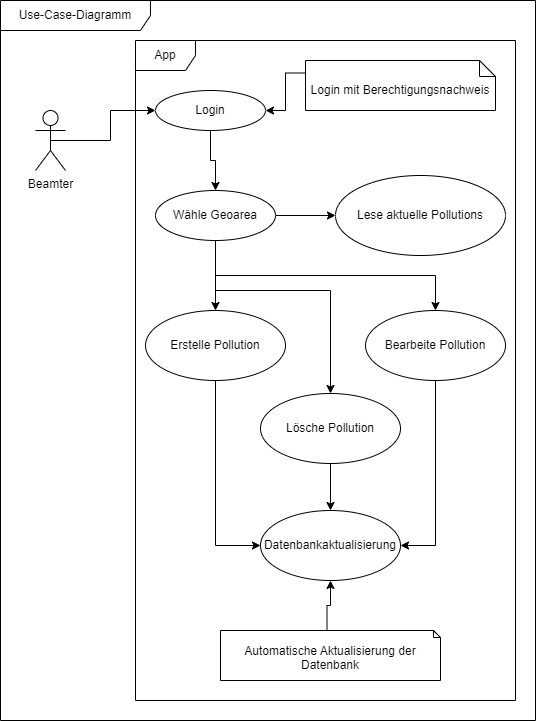
\includegraphics[width=0.9\textwidth]{bilder/use-case-diagramm.drawio.png}
\caption{Use-Case-Diagramm der \glqq Pollution Detection\grqq{}-App}
\end{figure}

\clearpage
\subsection{Lastenheft}
\label{sec:lastenheft}

Für die Entwicklung der \glqq Pollution Detection\grqq{}-App für die Polizeibehörde sind folgende Anforderungen festgelegt:\\

\noindent\textbf{1. Datenverarbeitung und Integration}

\begin{itemize}
    \item Die App \textbf{muss} Verschmutzungsdaten in Echtzeit erfassen und kategorisieren.
    \item Es \textbf{muss} möglich sein, spezifische \glspl{pollution} hinzuzufügen, die für bestimmte \glspl{geoarea} relevant sind.
    \item Es \textbf{muss} eine Funktion geben, die den Beamten erlaubt, \glspl{pollution} zu bearbeiten und zu löschen.
    \item Die erfassten Daten \textbf{könnten} mit anderen Datenquellen oder Systemen der Polizeibehörde synchronisiert werden.
\end{itemize}

\noindent\textbf{2. Benutzeroberfläche und Interaktivität}

\begin{itemize}
    \item Die App \textbf{muss} über eine intuitive Benutzeroberfläche verfügen, die eine schnelle und einfache Erfassung von \glspl{pollution} ermöglicht.
    \item Die App \textbf{könnte} in der Lage sein, die genaue Position der \gls{pollution} mithilfe von GPS oder anderen geografischen Tools zu erfassen.
\end{itemize}

\noindent\textbf{3. Zugänglichkeit}

\begin{itemize}
    \item Die App \textbf{muss} auf Mobilgeräten funktionieren.
    \item Die App \textbf{sollte} eine sichere Authentifizierungsmethode haben.
\end{itemize}

\noindent\textbf{4. Sonstige Anforderungen}

\begin{itemize}
    \item Es \textbf{sollten} regelmäßige Updates und Wartungen durchgeführt werden, um die App auf dem neuesten Stand zu halten und Sicherheitsrisiken zu minimieren.
    \item Es \textbf{wäre} gut, über kontinuierlichen Support und mögliche Einweisungen zu verfügen.
\end{itemize}

\clearpage
\subsection{Komponentendiagramm}
\label{sec:komponentendiagramm}

\begin{figure}[h]
\centering
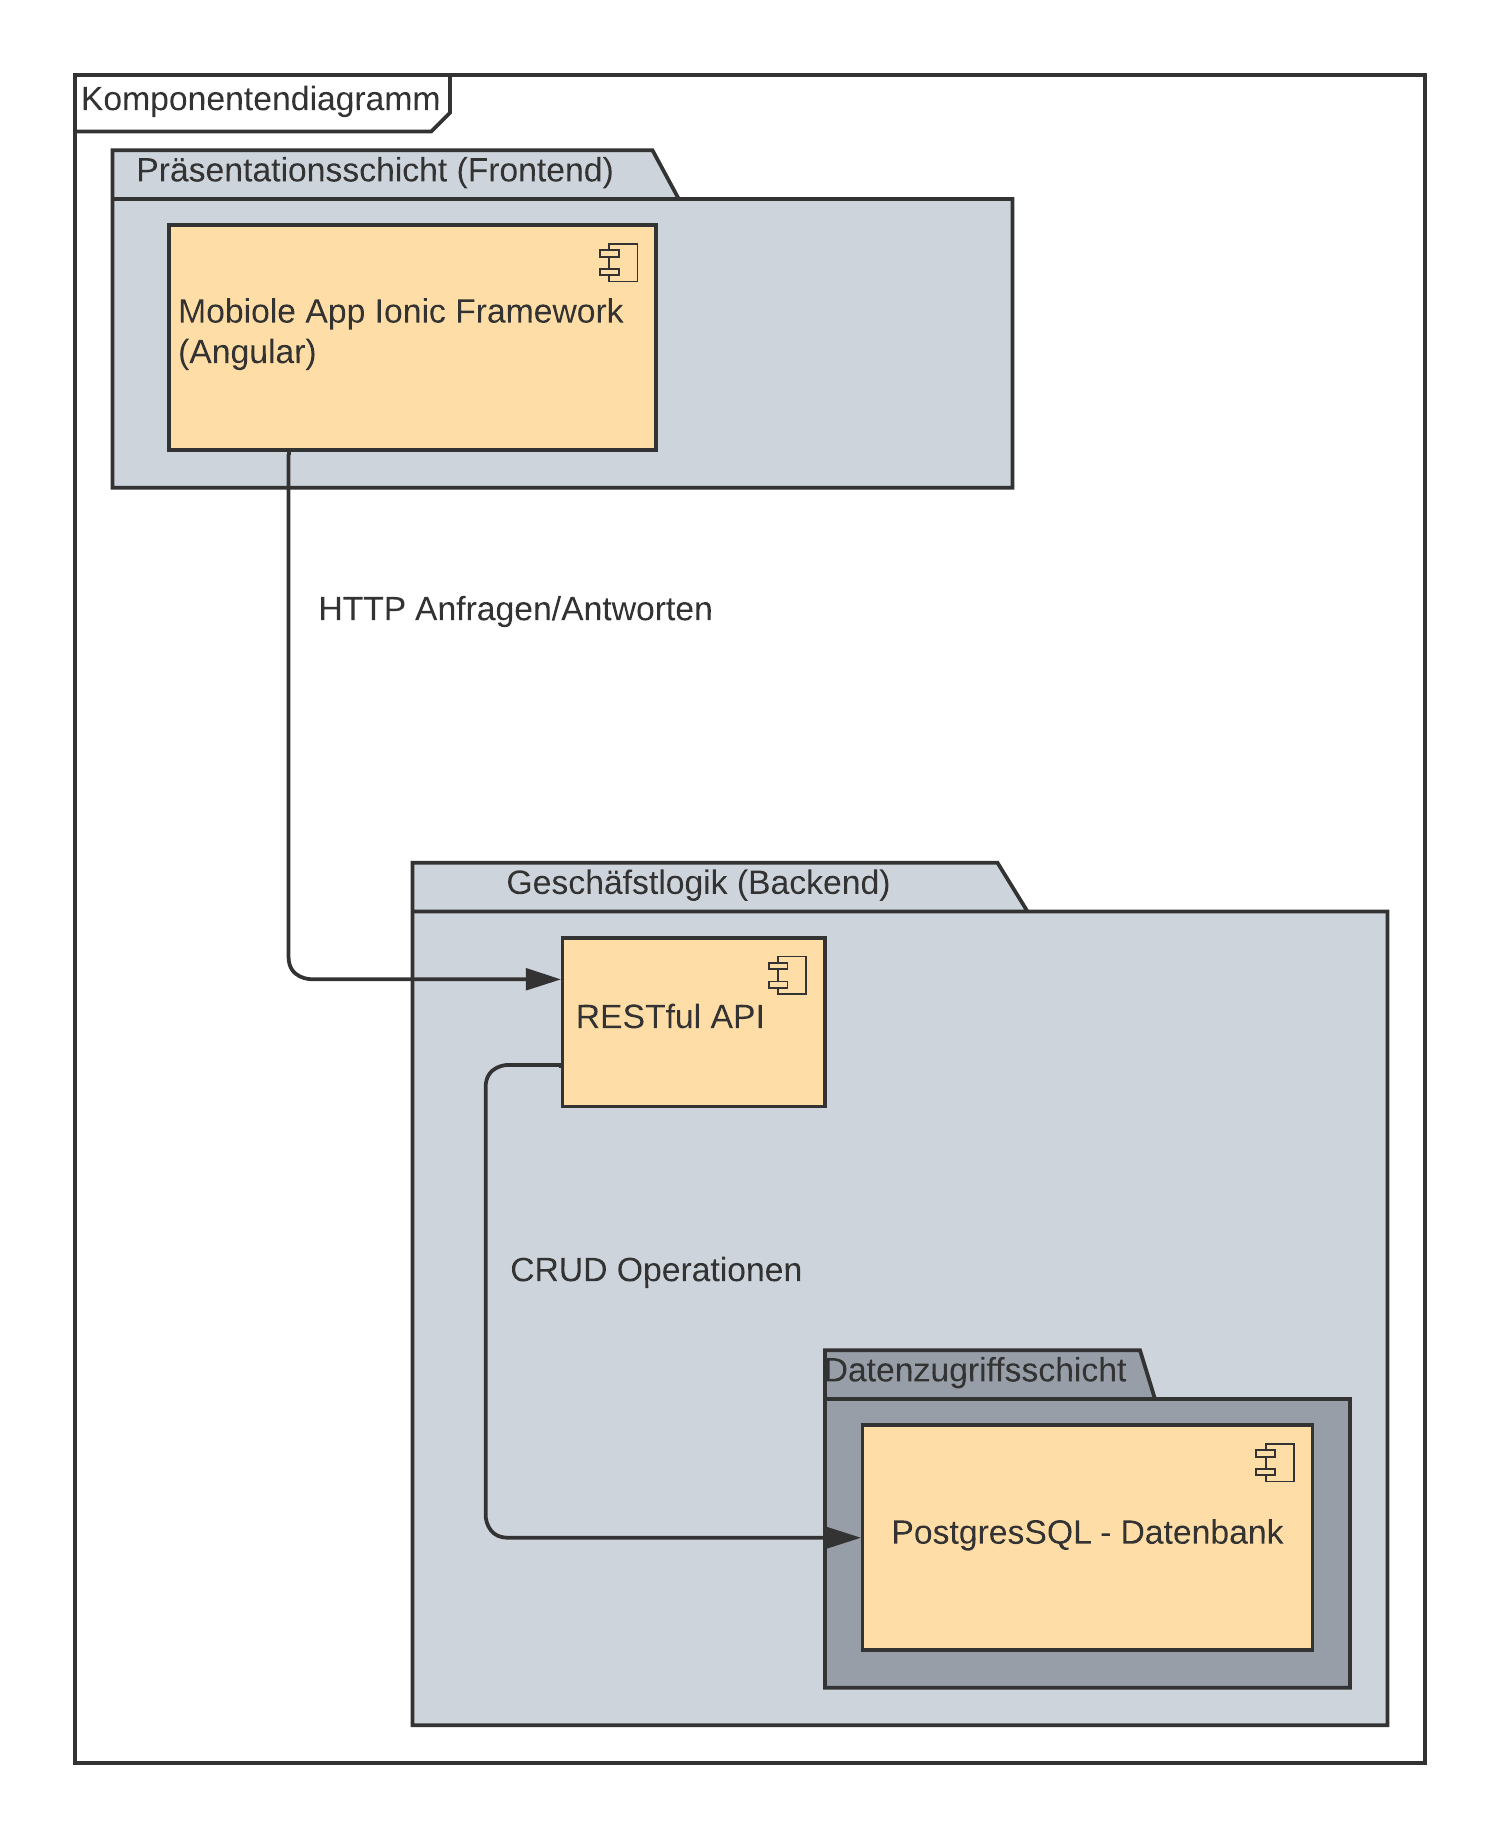
\includegraphics[width=0.9\textwidth]{bilder/Komponentendiagramm2.png}
\caption{Komponentendiagramm}
\end{figure}

\clearpage
\subsection{Mockups}
\label{sec:mockups}

\begin{figure}[h]
\centering
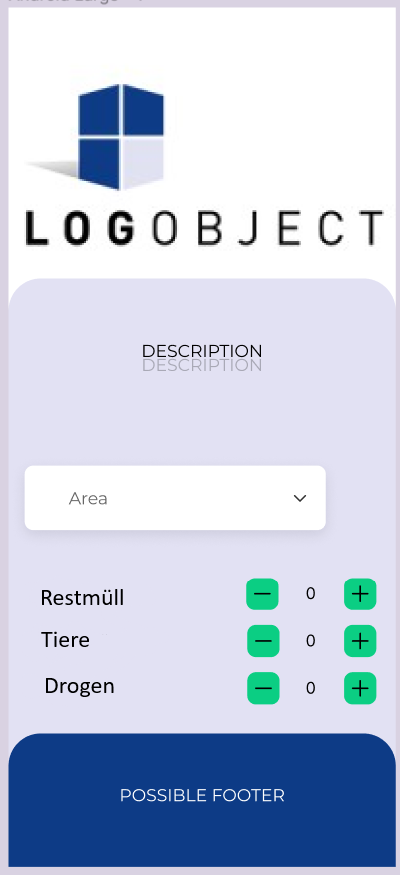
\includegraphics[width=0.5\textwidth]{bilder/prototyp1.png}
\caption{Mockups}
\end{figure}

\clearpage
\subsection{Entity-Relationship-Modell}
\label{sec:entity-relationship-modell}

\begin{figure}[h]
\centering
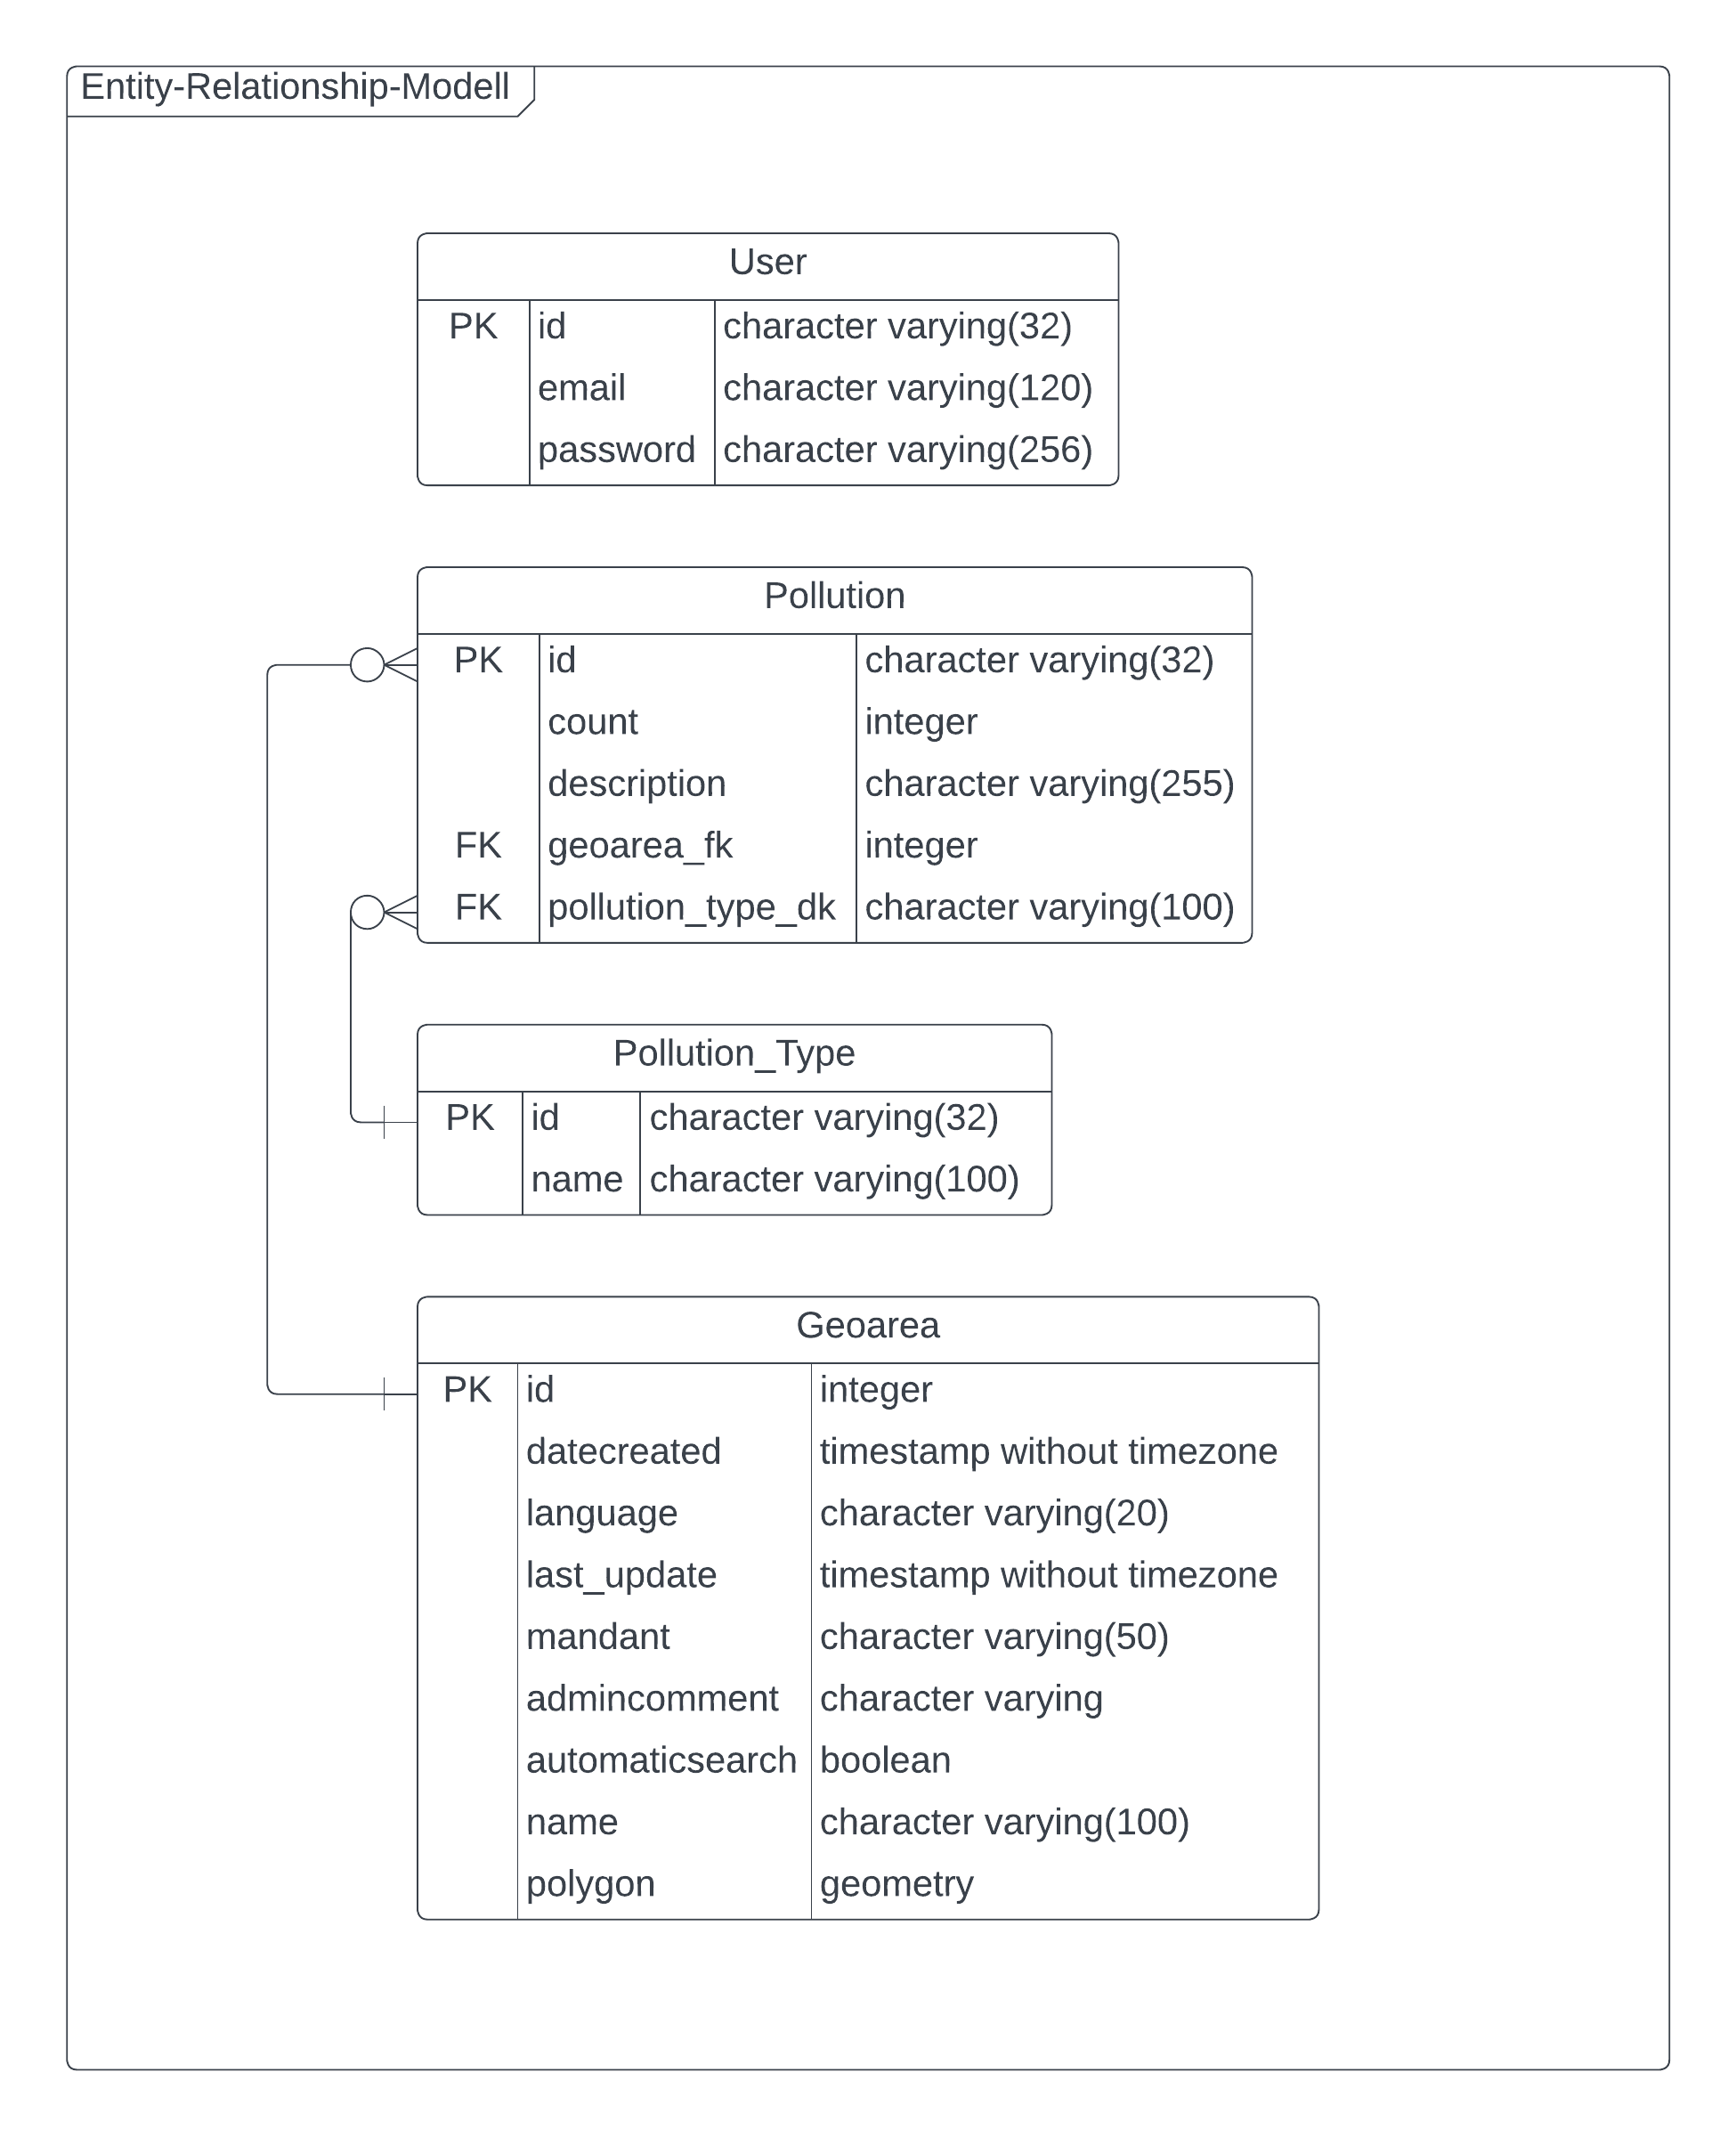
\includegraphics[width=0.9\textwidth]{bilder/Entity-Relationship-Diagram4.png}
\caption{Entity-Relationship-Modell}
\end{figure}

\clearpage
\subsection{Klassendiagramm (Auszug)}
\label{sec:klassendiagramm}

\begin{figure}[h]
\centering
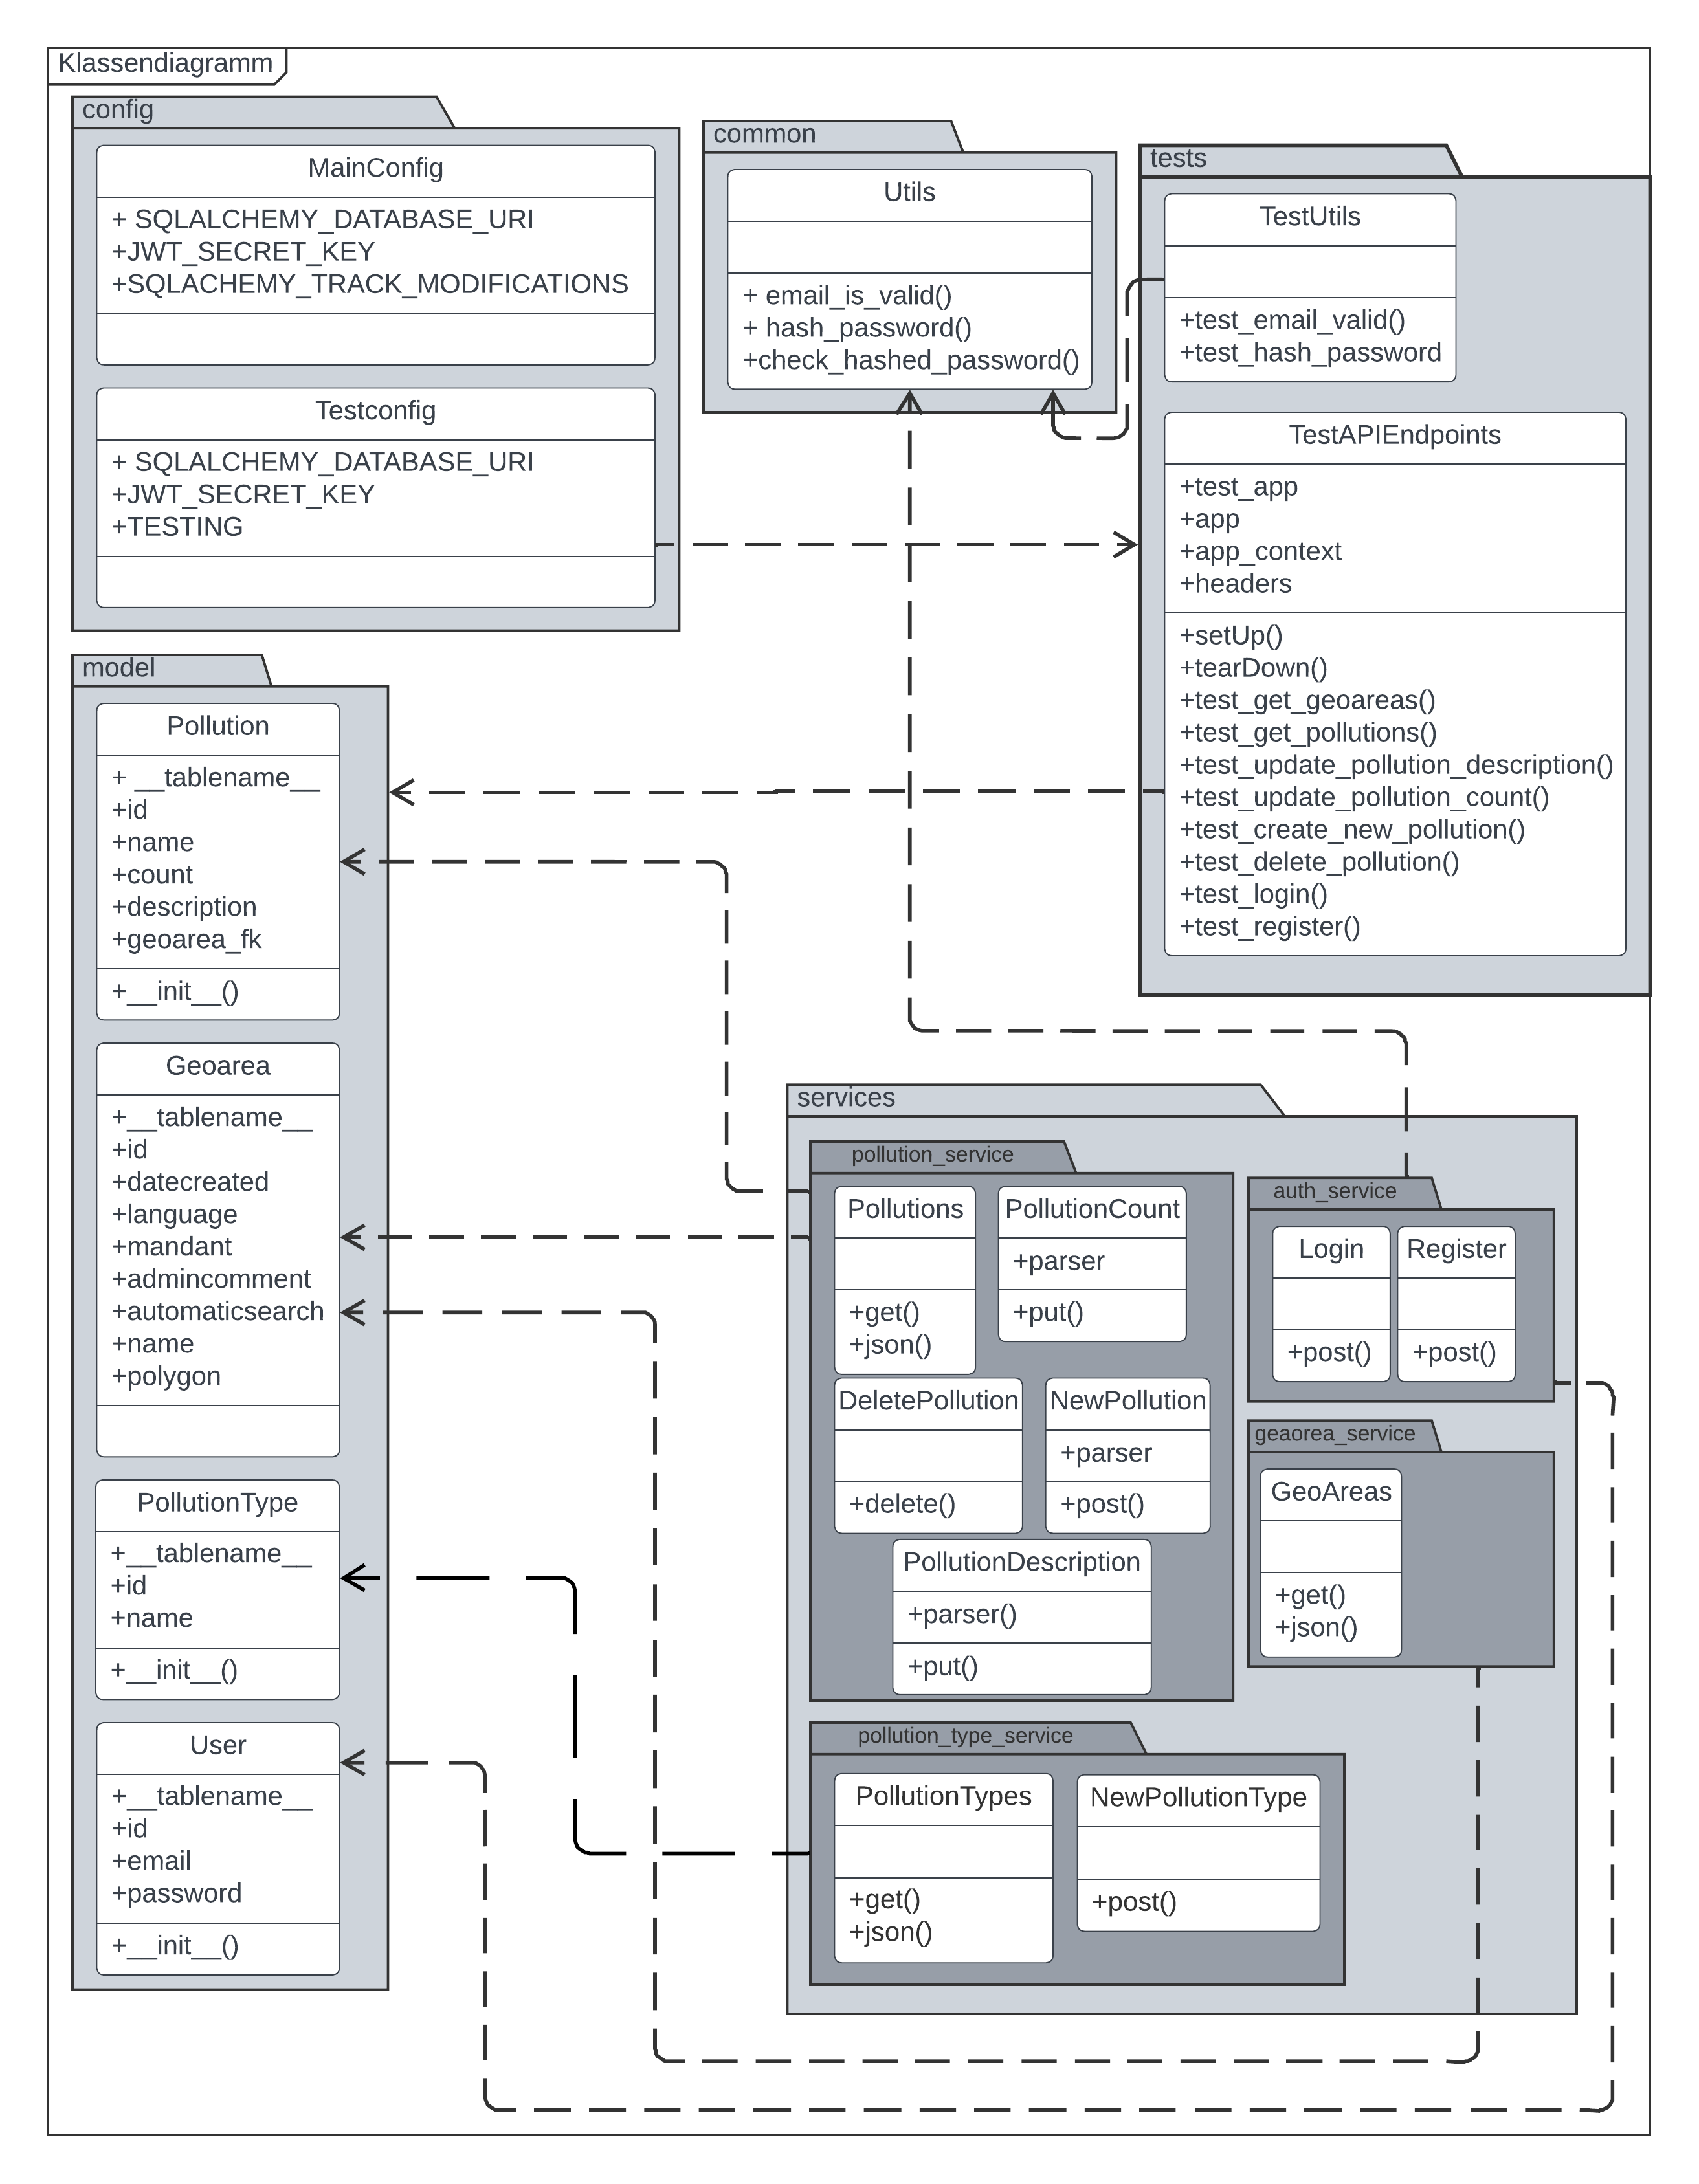
\includegraphics[width=0.8\textwidth]{bilder/klassendiagramm.png}
\caption{Auszug des Klassendiagramms}
\end{figure}

\clearpage
\subsection{Pflichtenheft (Auszug)}
\label{sec:pflichtenheft}

Der folgende Abschnitt bietet einen Auszug aus dem Pflichtenheft und beschreibt die geplante Umsetzung der im Lastenheft definierten Anforderungen:\\
\\
\noindent\textbf{1. Entwicklungsumgebung und Plattform}
\begin{itemize}
    \item Als Entwicklungsumgebung wird \acrshort{vscode} verwendet.
    \item Die \acrshort{api} wird mit \acrshort{python3} unter Verwendung des Flask-Frameworks entwickelt.
    \item Es wird eine Schnittstelle implementiert, über die Verschmutzungsdaten erfasst, kategorisiert, bearbeitet und gelöscht werden können.
    \item Die Anwendung wird auf einem Laptop im firmeninternen Netzwerk deployed und dort getestet.
    \item Für die \acrshort{ci} wird GitHub Actions eingesetzt.
\end{itemize}

\noindent\textbf{2. Datenbank}
\begin{itemize}
    \item Die Daten werden in einer Postgres-Testdatenbank gespeichert.
    \item Sowohl die Datenbank als auch die \acrshort{api} werden in Docker-Containern gehostet.
\end{itemize}

\noindent\textbf{3. Oberfläche und Interaktivität}
\begin{itemize}
    \item Für die Entwicklung der App-Oberfläche wird das Ionic Framework auf Basis von Angular verwendet.
    \item Die Benutzeroberfläche wird für eine schnelle Erfassung von \glspl{pollution} optimiert.
    \item Die Oberfläche wird automatisch gebaut und in eine native App umgewandelt.
\end{itemize}

\noindent\textbf{4. Zugänglichkeit und Sicherheit}
\begin{itemize}
    \item Die App wird für Mobilgeräte optimiert.
    \item Es wird eine Authentifizierungsmethode implementiert.
\end{itemize}

\noindent\textbf{5. Geschäftslogik, Tests und Wartung}
\begin{itemize}
    \item Für die \gls{api} werden Unittests in Python durchgeführt.
    \item Ein regelmäßiges Update- und Wartungssystem wird eingerichtet.
    \item Ein Support-System wird bereitgestellt.
\end{itemize}

\clearpage
\subsection{Listing von Python-Code}
\subsubsection{Datenmodelle und Services}
\label{sec:python-code}
\lstset{
  basicstyle=\rmfamily\small,
  backgroundcolor=\color{paleyellow},
  commentstyle=\color{graugruen},
  keywordstyle=\color{darkblue},
  stringstyle=\color{codepurple},
  breakatwhitespace=false,
  breaklines=true,
  captionpos=b,
  keepspaces=true,
  numbers=left,
  numbersep=10pt,
  showspaces=false,
  showstringspaces=false,
  showtabs=false,
  tabsize=4,
  columns=flexible,
  frame=single
}

\begin{lstlisting}[language=Python, caption=Implementation der Pollution-Klasse, label=lst:pollution]
class Pollution(db.Model):
    __tablename__ = 'pollution'

    id = db.Column(
        db.String(32), primary_key=True, unique=True, nullable=False,
        default=lambda: uuid.uuid4().hex)
    count = db.Column(db.Integer)
    description = db.Column(db.String)
    geoarea_fk = db.Column(db.Integer, db.ForeignKey('geoarea.id'))
    pollution_type_fk = db.Column(db.String, db.ForeignKey('pollution_type.id'))
\end{lstlisting}

\begin{lstlisting}[language=Python, caption=Implementation der PollutionCount-Klasse, label=lst:pollutionCount]
class PollutionCount(Resource):
    parser = reqparse.RequestParser()
    parser.add_argument('count', type=int, required=True, help="Count field is required")

    @jwt_required()
    def put(self, pollution_id: str):
        data = PollutionCount.parser.parse_args()
        pollution = Pollution.query.get(pollution_id)

        if not pollution:
            return {"message": "Pollution not found"}, 404

        pollution.count = data['count']

        try:
            db.session.commit()  # Commit the changes to the database
            return {"message": "PollutionCount updated successfully"}, 200
        except Exception as e:
            db.session.rollback()  # Rollback changes in case of an error
            return {"message": f"An error occurred while updating pollution: {str(e)}"}, 500
\end{lstlisting}

\clearpage
\subsubsection{Listing von unittest}
\label{sec:unittest}
\lstset{
  basicstyle=\rmfamily\small,
  backgroundcolor=\color{paleyellow},
  commentstyle=\color{graugruen},
  keywordstyle=\color{darkblue},
  stringstyle=\color{codepurple},
  breakatwhitespace=false,
  breaklines=true,
  captionpos=b,
  keepspaces=true,
  numbers=left,
  numbersep=10pt,
  showspaces=false,
  showstringspaces=false,
  showtabs=false,
  tabsize=4,
  columns=flexible,
  frame=single
}

\begin{lstlisting}[language=Python, caption=Implementation der Utils-Tests, label=lst:utilstest]
import unittest
from common.utils import Utils

class TestUtils(unittest.TestCase):
    def test_email_valid(self):
        self.assertTrue(Utils.email_is_valid("example@example.com"))
        self.assertFalse(Utils.email_is_valid("invalid_email"))

    def test_hash_password(self):
        password = "password123"
        hashed_password = Utils.hash_password(password)
        self.assertTrue(Utils.check_hashed_password(password, hashed_password))
        self.assertFalse(Utils.check_hashed_password("wrong_password", hashed_password))


if __name__ == '__main__':
    unittest.main()
\end{lstlisting}

\begin{lstlisting}[language=Python, caption=Implementation der Integrationstests , label=lst:integrationtest]
class TestAPIEndpoints(unittest.TestCase):
    def setUp(self):
        print("start setting up test environment...")

        warnings.filterwarnings("ignore")

        self.test_app = create_app(TestConfig, db)
        self.app = self.test_app.test_client()

        self.app_context = self.test_app.app_context()
        self.app_context.push()

        # Create the tables using the application context
        with self.test_app.app_context():
            db.create_all()

    def tearDown(self):
        # Drop the tables using the application context
        with self.test_app.app_context():
            print("tearDown")
            db.session.close_all()
            db.drop_all()

        self.app_context.pop()

    def test_update_pollution_count(self):
        geoarea = GeoArea(
            id=5,
            name='Area 5',
            datecreated='2023-01-01 00:00:00',
            language='German',
            last_update='2023-08-25 00:00:00',
            mandant='Mandant A',
            admincomment='Comment 1',
            automaticsearch=True,
            polygon="POLYGON((1 2,2 3, 3 4, 5 6, 1 2))"
        )

        pollutionType1 = PollutionType(
            name='Typ 1'
        )
        db.session.add(pollutionType1)
        db.session.commit()

        pollution = Pollution(
            count=10,
            description='Description 1',
            geoarea_fk=5,
            pollution_type_fk=db.session.query(PollutionType).first().id
        )
        db.session.add_all([pollutionType1, pollution, geoarea])
        db.session.commit()

        expires = timedelta(days=7)
        access_token = create_access_token(identity=geoarea.id, expires_delta=expires)
        self.headers = {'Authorization': f'Bearer {access_token}'}

        with self.test_app.test_client() as client:
            response = client.put('/pollution/pollutionCount/' + pollution.id,
                                  json={'count': 15}, headers=self.headers)

            self.assertEqual(response.status_code, 200)

            updated_pollution = db.session.query(Pollution).get(pollution.id)
            self.assertEqual(updated_pollution.count, 15)
\end{lstlisting}

\clearpage
\subsection{Benutzerdokumentation (Auszug)}
\label{sec:benutzerdokumentation}
Nach erfolgreicher Anmeldung gelangen Sie zur Hauptseite.

\begin{figure}[h]
\centering
\includegraphics[width=0.4\textwidth]{bilder/select\_geoarea.png}
\end{figure}

\noindent Hier befindet sich ein Dropdown-Menü mit der Beschriftung \glqq Select geoarea\grqq{}. Um eine Geoarea auszuwählen, klicken Sie auf die Leiste. Es öffnet sich ein Menü mit den verfügbaren Geoareas. Wählen Sie die gewünschte \gls{geoarea} aus, um die \glspl{pollution} zu dem ausgewählten Gebiet zu erhalten.

\begin{figure}[h]
\centering
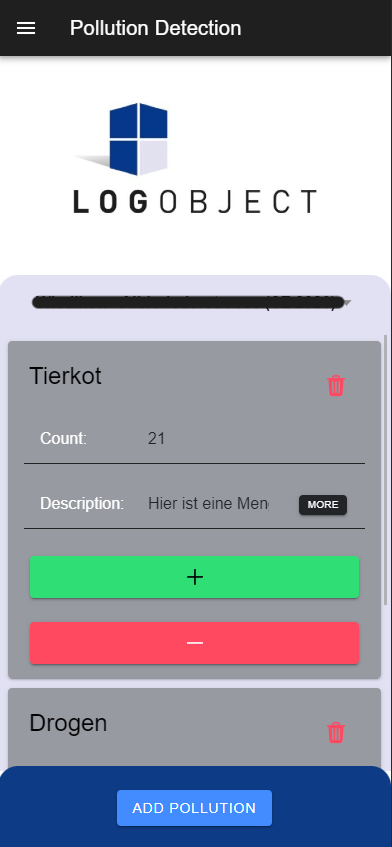
\includegraphics[width=0.365\textwidth]{bilder/pollutions1.png}
\end{figure}

\noindent Hier können Sie verschiedene Aktionen durchführen:

\begin{enumerate}
    \item \textbf{Anzahl bearbeiten:} Jede \gls{pollution} zeigt die aktuelle Anzahl (Count) an. Mit den Plus- und Minus-Tasten können Sie die Anzahl der jeweiligen \gls{pollution} erhöhen oder verringern.
    \item \textbf{Beschreibung bearbeiten:} Um die Beschreibung einer \gls{pollution} zu ändern, klicken Sie einfach auf das Beschreibungsfeld. 
    \item \textbf{Mehr anzeigen:} Wenn der Beschreibungstext zu lang ist und nicht vollständig angezeigt wird, klicken Sie auf den \glqq More\grqq{}-Button. Ein Pop-Up-Fenster erscheint, in dem die vollständige Beschreibung sichtbar ist.
   \item \textbf{\gls{pollution} löschen:} Das kleine Mülleimer-Symbol in der oberen rechten Ecke jeder \gls{pollution} dient dazu, den Löschvorgang zu initiieren. Ein Klick darauf öffnet ein kleines Fenster, das nach einer Bestätigung fragt, um sicherzustellen, dass Sie die \gls{pollution} tatsächlich löschen möchten. Erst nach der Bestätigung wird die \gls{pollution} endgültig gelöscht.
    \item \textbf{Neue \gls{pollution} hinzufügen:} Unten befindet sich ein Button mit der Bezeichnung \glqq ADD POLLUTION\grqq{}. Wenn Sie diesen anklicken, öffnet sich ein Menü, in dem Sie eine neue \gls{pollution} für das ausgewählte Gebiet hinzufügen können.
\end{enumerate}

\begin{figure}[h]
\centering
\includegraphics[width=0.5\textwidth]{bilder/add\_pollution.png}
\end{figure}

\noindent In diesem Menü können Sie eine neue \gls{pollution} zur aktuell ausgewählten Geoarea hinzufügen. Es ist wichtig, dass bereits eine Geoarea ausgewählt wurde und dass die neue \gls{pollution} einen eindeutigen Type besitzt. Ohne diese Informationen ist das Hinzufügen einer neuen \gls{pollution} nicht möglich.:
\begin{enumerate}
    \item \textbf{\gls{pollutiontype}:} Wählen Sie den Type der neuen \gls{pollution} im Feld \glqq Pollution Type\grqq{} aus.
    \item \textbf{Anzahl:} Setzen Sie die Anzahl der \gls{pollution}, standardmäßig auf 0 gesetzt.
    \item \textbf{Beschreibung:} Fügen Sie eine detaillierte Beschreibung der \gls{pollution} im Feld \glqq Description\grqq{} hinzu.
    \item \textbf{Bestätigen oder Abbrechen:} Klicken Sie auf \glqq CONFIRM\grqq{}, um die \gls{pollution} hinzuzufügen, oder auf \glqq CANCEL\grqq{}, um das Hinzufügen abzubrechen.
\end{enumerate}

\clearpage
\subsection{Entwicklerdokumentation (Auszug)}
\label{sec:entwicklerdokumentation}

\begin{figure}[h]
\centering
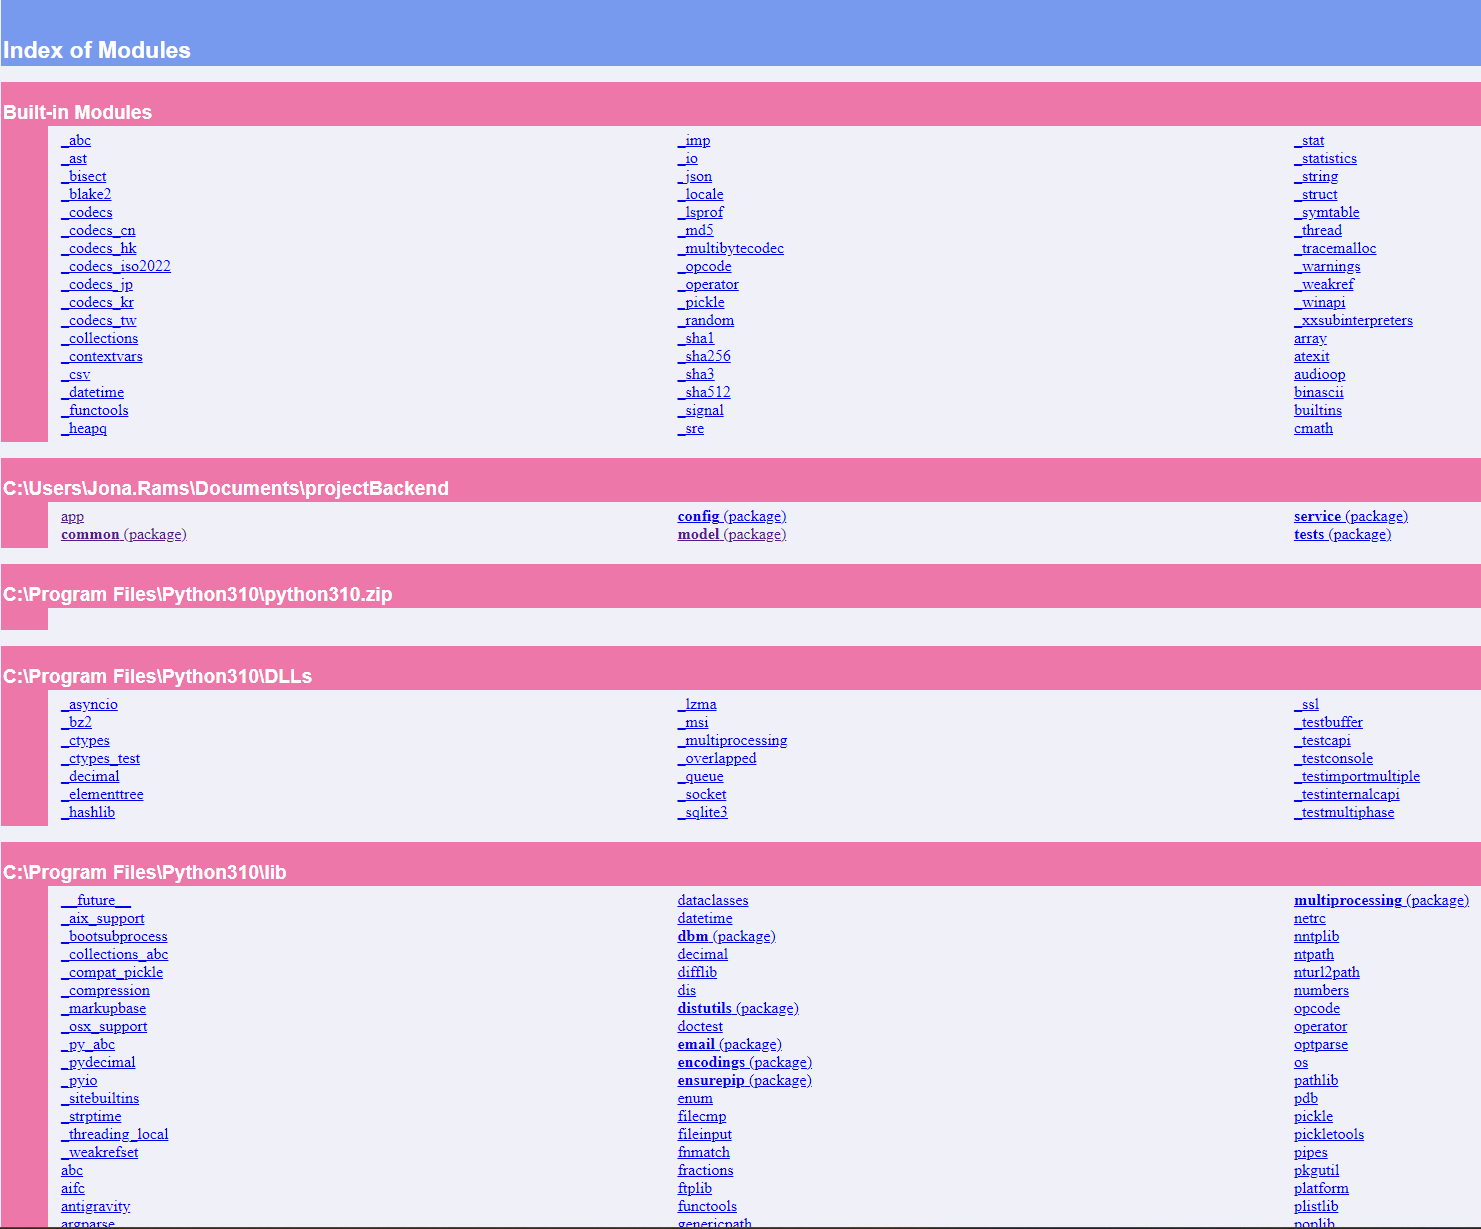
\includegraphics[width=1\textwidth]{bilder/entwicklerdokumentation.png}
\caption{Startseite der Entwicklerdokumentation}
\end{figure}

\begin{figure}[h]
\centering
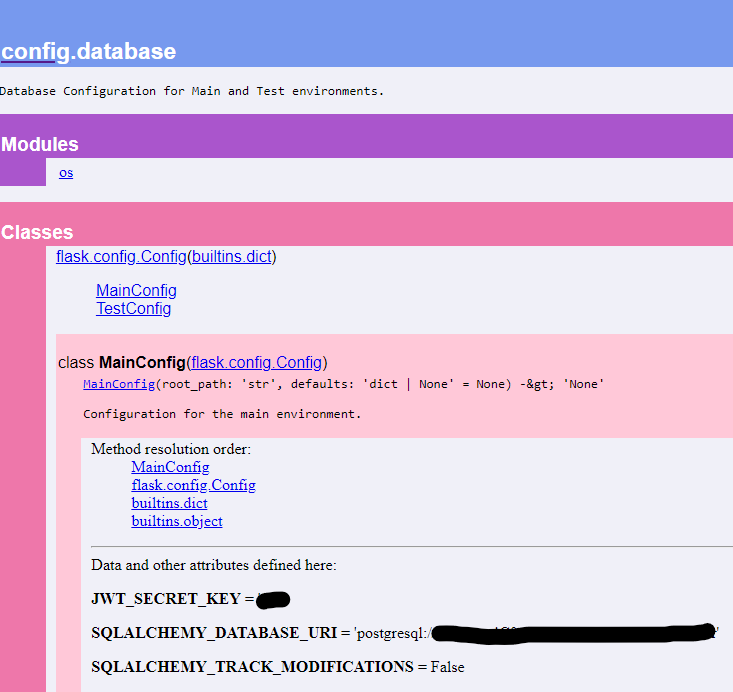
\includegraphics[width=1\textwidth]{bilder/databasedoku.png}
\caption{Entwicklerdokumentation der Datenbankkofiguration}
\end{figure}

\end{document}